%%%%%%%%%%%%%%%%%%%%%%%%%%%%%%%%%%%%%%%%%%%%%%%%%%%%%%%%%%%%%%%%%%%%%%%%%%%%%%%%
%%%%%%%%%%%%%%%%%%   Vorlage für eine Abschlussarbeit   %%%%%%%%%%%%%%%%%%%%%%%%
%%%%%%%%%%%%%%%%%%%%%%%%%%%%%%%%%%%%%%%%%%%%%%%%%%%%%%%%%%%%%%%%%%%%%%%%%%%%%%%%

% Erstellt von Maximilian Nöthe, <maximilian.noethe@tu-dortmund.de>
% ausgelegt für lualatex und Biblatex mit biber

% Kompilieren mit
% latexmk --lualatex --output-directory=build thesis.tex
% oder einfach mit:
% make

\documentclass[
  tucolor,       % remove for less green,
  BCOR=12mm,     % 12mm binding corrections, adjust to fit your binding
  parskip=half,  % new paragraphs start with half line vertical space
  open=any,      % chapters start on both odd and even pages
  cleardoublepage=plain,  % no header/footer on blank pages
]{tudothesis}


% Warning, if another latex run is needed
\usepackage[aux]{rerunfilecheck}

% just list chapters and sections in the toc, not subsections or smaller
\setcounter{tocdepth}{1}

%------------------------------------------------------------------------------
%------------------------------ Fonts, Unicode, Language ----------------------
%------------------------------------------------------------------------------
\usepackage{fontspec}
\defaultfontfeatures{Ligatures=TeX}  % -- becomes en-dash etc.

% load english (for abstract) and ngerman language
% the main language has to come last
\usepackage[ngerman, american]{babel}

% intelligent quotation marks, language and nesting sensitive
\usepackage[autostyle]{csquotes}

% microtypographical features, makes the text look nicer on the small scale
\usepackage{microtype}

%------------------------------------------------------------------------------
%------------------------ Math Packages and settings --------------------------
%------------------------------------------------------------------------------

\usepackage{amsmath}
\usepackage{amssymb}
\usepackage{mathtools}

% Enable Unicode-Math and follow the ISO-Standards for typesetting math
\usepackage[
  math-style=ISO,
  bold-style=ISO,
  sans-style=italic,
  nabla=upright,
  partial=upright,
  warnings-off={mathtools-colon,mathtools-overbracket}, % suppress some unnecessary warnings
]{unicode-math}
\setmathfont{Latin Modern Math}

% nice, small fracs for the text with \sfrac{}{}
\usepackage{xfrac}


%------------------------------------------------------------------------------
%---------------------------- Numbers and Units -------------------------------
%------------------------------------------------------------------------------

\usepackage[
  locale=US,
  separate-uncertainty=true,
  per-mode=symbol-or-fraction,
]{siunitx}
% Lightspeed as a unit
\DeclareSIUnit{\lightspeed}{\text{\ensuremath{c}}}

%------------------------------------------------------------------------------
%-------------------------------- tables  -------------------------------------
%------------------------------------------------------------------------------

\usepackage{tabularray}
\usepackage{booktabs}       % \toprule, \midrule, \bottomrule, etc
\UseTblrLibrary{booktabs, siunitx}

%------------------------------------------------------------------------------
%-------------------------------- graphics -------------------------------------
%------------------------------------------------------------------------------

\usepackage{graphicx}
% currently broken
% \usepackage{grffile}

% allow figures to be placed in the running text by default:
\usepackage{scrhack}
\usepackage{float}
\floatplacement{figure}{htbp}
\floatplacement{table}{htbp}

% keep figures and tables in the section
\usepackage[section, below]{placeins}

% allows to include PDFs as full pages
\usepackage{pdfpages}

% Set the PDF Version of this document to 1.7 (1.4 is the current default)
% This is needed so that PDFs with Version >1.5 can be included
\pdfvariable minorversion=7

% for drawing Feynman diagrams
\usepackage{tikz}
\usepackage[compat=1.1.0]{tikz-feynman}

%------------------------------------------------------------------------------
%---------------------- customize list environments ---------------------------
%------------------------------------------------------------------------------

\usepackage{enumitem}

%------------------------------------------------------------------------------
%------------------------------ Bibliographie ---------------------------------
%------------------------------------------------------------------------------

\usepackage[
  backend=biber,   % use modern biber backend
  autolang=hyphen, % load hyphenation rules for if language of bibentry is not
                   % german, has to be loaded with \setotherlanguages
                   % in the references.bib use langid={en} for english sources
  sorting=none,
]{biblatex}
\addbibresource{references.bib}  % the bib file to use
\DefineBibliographyStrings{german}{andothers = {{et\,al\adddot}}}  % replace u.a. with et al.


% Last packages, do not change order or insert new packages after these ones
\usepackage[pdfusetitle, unicode, linkbordercolor=tugreen, citebordercolor=tugreen]{hyperref}
\usepackage{bookmark}
\usepackage[shortcuts]{extdash}
\usepackage[capitalise]{cleveref}

%------------------------------------------------------------------------------
%-------------------------    Angaben zur Arbeit   ----------------------------
%------------------------------------------------------------------------------

\author{Pascal Maximilian Machnik}
\title{Measurement of Beauty Baryon Decays at the LHCb Experiment}
\date{2025}
\birthplace{Hagen}
\chair{Arbeitsgruppe Albrecht}
\division{Fakultät Physik}
\thesisclass{Bachelor of Science}
\submissiondate{21. August 2025}
\firstcorrector{Prof.~Dr.~Johannes Albrecht}
\secondcorrector{Prof.~Dr.~Kevin Alexander Kröninger}

% tu logo on top of the titlepage
\titlehead{
\includegraphics[height=1.5cm]{logos/tu-logo.pdf}}

\begin{document}
\frontmatter
\maketitle

% Gutachterseite
\makecorrectorpage

% hier beginnt der Vorspann, nummeriert in römischen Zahlen
\thispagestyle{plain}

\section*{Abstract}
In this thesis, the rare baryonic decay $\Lambda_b^0 \to \Lambda^0 \mu^+ \mu^-$ is measured for the first time using Run 3 data collected by the LHCb experiment in 2024. The corresponding Run 2 dataset is also analyzed, providing a baseline to assess how the LHCb detector and trigger upgrades for Run 3 affect the analysis of rare baryonic decays. Because of its relatively long lifetime, the neutral $\Lambda^0$ hyperon can decay either inside or outside the Vertex Locator (VELO), resulting in long tracks, which include hits in the VELO, or downstream tracks, which do not. Signal candidates are classified as Long--Long (LL) or Downstream--Downstream (DD), depending on the track types of both $\Lambda^0$ decay products. To account for differences in reconstruction, LL and DD events are analyzed separately. 

The measured Run 3 signal yields are lower relative to Run 2, partly due to the lack of simulation calibration and selection optimization in the Run 3 study. The reduction is especially pronounced for DD events, likely reflecting the commissioning status of the Upstream Tracker during the Run 3 data taking.
%The relatively long lifetime of the neutral $\Lambda^0$ hyperon can cause its decay products to originate beyond the Vertex Locator (VELO), resulting in long tracks, which include hits in the VELO, or downstream tracks, which do not.
%This thesis presents the first measurement of the rare baryonic decay $\Lambda_b^0 \to \Lambda^0 \mu^+ \mu^-$ using Run 3 data collected by the LHCb data, while also studying the corresponding Run 2 dataset to assess the impact of Upgrade I on the analysis of rare baryonic decays.
%This thesis presents the first measurement of the rare baryonic decay $\Lambda_b^0 \to \Lambda^0 \mu^+ \mu^-$ using data collected by the LHCb experiment during Run 3 of the LHC, providing a complementary perspective to the mesonic sector in the study of $B$-anomalies.
%By comparing the yields obtained in both runs, this study assesses the impact of the Run 3 detector and trigger upgrades on the analysis of rare baryonic decays. 
%The signal yield in Run 3 is observed to be reduced compared to Run 2. This reduction is partly due to the absence of simulation calibration and offline selection optimization, which results in suboptimal selection performance. The reduction is particularly pronounced in the DD category, likely reflecting the impact of the Upstream Tracker, which was still in the installation and commissioning phase during Run 3 data taking.

\section*{Kurzfassung}
\begin{foreignlanguage}{german}
In dieser Arbeit wird der seltene baryonische Zerfall $\Lambda_b^0 \to \Lambda^0 \mu^+ \mu^-$ erstmals mit Run‑3-Daten des LHCb-Experiments aus dem Jahr 2024 gemessen. Die entsprechenden Run‑2-Daten werden ebenfalls analysiert und dienen als Referenz, um zu bewerten, wie sich die für Run 3 durchgeführten Detektor- und Trigger‑Upgrades am LHCb-Experiment auf die Analyse seltener baryonischer Zerfälle auswirken. Aufgrund seiner relativ langen Lebensdauer kann das neutrale $\Lambda^0$-Hyperon entweder innerhalb oder außerhalb des Vertex Locators (VELO) zerfallen. Dies führt zu long tracks, die Spuren im VELO hinterlassen, oder zu downstream tracks, bei denen diese Spuren ausbleiben. Signalkandidaten werden dementsprechend, abhängig von den Spurtypen beider $\Lambda^0$-Zerfallsprodukte, in Long-Long (LL)- oder Downstream-Downstream (DD)-Ereignisse klassifiziert. Um Unterschiede in der Rekonstruktion zu berücksichtigen, werden LL- und DD-Ereignisse separat analysiert.

Die in Run 3 gemessene Anzahl an Signalzerfällen fällt im Vergleich zu Run 2 geringer aus. Dieser Effekt ist zum Teil auf die bislang fehlende Simulationskalibrierung sowie die noch nicht optimierte Selektion der Run-3-Studie zurückzuführen. Besonders ausgeprägt ist die Reduktion bei DD-Ereignissen, was vermutlich den Inbetriebnahmestatus des Upstream-Trackers während der Datennahme in Run 3 widerspiegelt.
\end{foreignlanguage}


%Die relativ lange Lebensdauer des neutralen $\Lambda^0$-Hyperons kann dazu führen, dass seine Zerfallsprodukte außerhalb des Vertex Locators (VELO) entspringen. Dies resultiert entweder in  long tracks, die im VELO Spuren hinterlassen, oder in downstream tracks, bei denen diese Spuren ausbleiben.
%Diese Arbeit präsentiert die erste Run-3-Messung des seltenen baryonischen Zerfalls $\Lambda_b^0 \to \Lambda^0 \mu^+ \mu^-$ am LHCb-Experiment und eröffnet damit eine komplementäre Perspektive zum mesonischen Sektor bei der Untersuchung von $B$-Anomalien.Zusätzlich werden Daten aus Run 2 herangezogen, um einen direkten Vergleich zwischen den beiden Datennahmeperioden zu ermöglichen.

%In doing so, events are classified as Long--Long (LL) or Downstream-Downstream (DD), depending on the track types of both decay products of the $\Lambda^0$ hyperon.

\tableofcontents

\mainmatter
% Hier beginnt der Inhalt mit Seite 1 in arabischen Ziffern
\chapter{Introduction}
\label{ch:introduction}
The Standard Model of particle physics (SM) \cite{salam1959,glashow1959,weinberg1967} is a very successful theory, confirmed by many experimental measurements. However, several observations, such as non-zero neutrino masses \cite{neutrino_osc}, are not yet explained within the SM, motivating the search for New Physics (NP). Rare decays, which are strongly suppressed in the SM, are highly sensitive to potential NP contributions. As a result, they provide tests of SM predictions and enable the indirect search for NP.

Measurements of mesonic and baryonic decays involving the Flavor-Changing Neutral Current transition $b \to s \, \ell^+ \, \ell^-$ show such deviations from SM predictions \cite{b-anomalies_1, b-anomalies_2}, known as $B$-anomalies, which hint at possible NP contributions. Precision measurements of rare decays involving beauty quarks are a key focus of the LHCb experiment. During the second long shutdown of the Large Hadron Collider (LHC), LHCb underwent a major upgrade, referred to as Upgrade I \cite{lhcb_upgrade_I}, which replaced several subdetectors and introduced a fully software-based trigger system with new readout electronics.

The rare decay $\Lambda_b^0 \to \Lambda^0 \mu^+ \mu^-$ serves as a representative of the $b \to s \, \ell^+ \ell^-$ transition in the baryonic sector, providing complementary information on $B$-anomalies to that obtained from the extensively studied mesonic sector. So far, no study has been performed on this decay using Run 3 data. The aim of this thesis is to measure the signal yields for this rare decay with data collected by the LHCb experiment during Run 2 and Run 3 of the LHC, enabling a comparison between the two data-taking periods. Because of its relatively long lifetime, the $\Lambda^0$ hyperon may decay either inside or beyond the Vertex Locator (VELO), resulting in two different track types for its decay products: long tracks, which include hits in the VELO, and downstream tracks reconstructed without VELO information. This thesis analyzes the two event types separately to account for differences in reconstruction, thereby providing a more detailed understanding of the Run 3 data quality.

An introduction to the SM and the decay $\Lambda_b^0 \to \Lambda^0 \mu^+ \mu^-$ is given in \cref{ch:theory}. \cref{ch:lhcb} then presents an overview of the LHCb detector and Upgrade I. The analysis strategies for Run 2 and 3 are detailed in \cref{ch:run2} and \cref{ch:run3}, respectively. They contain online, offline, and multivariate selections, as well as the extraction of signal yields via invariant mass fits. A comparison between the two data-taking periods is performed. Finally, \cref{ch:conclusion} summarizes the results.

\chapter{Theoretical Foundation}
\label{ch:theory}
This chapter introduces the Standard Model of particle physics. It also discusses
the properties of the quark level transition $b \to s \, \mu^+ \, \mu^-$, which is the main mechanism for the rare decay 
$\Lambda_b^0 \to \Lambda^0 \, \mu^+ \, \mu^-$ studied in this thesis.


\section{The Standard Model of Particle Physics}
\label{sec:standard-model}
The SM \cite{salam1959,glashow1959,weinberg1967} is the theoretical framework that describes all currently known elementary particles and their interactions, except for gravitation. At present, it provides the most accurate description of the universe at the smallest scales. However, it does not yet account for several observed phenomena, such as the presence of dark matter \cite{rubin1970}. Therefore, the predictions of the SM need to be tested against experimental data in order to measure the free parameters of the SM and to search for NP.

\subsection{Elementary Particles}
\label{subsec:fundamental-particles}
The SM classifies all known elementary particles into bosons and fermions. Fermions are half-integer spin
particles that make up matter, while bosons are integer-spin particles that mediate forces between fermions, 
with the exception of the Higgs boson. 

Fermions are further divided into quarks and leptons, each having spin $\tfrac{1}{2}$. There are three 
generations of leptons, each containing a charged lepton with charge $-\,e$, quantified by the elementary 
charge $e$, and a corresponding massless and neutral neutrino:
\begin{align*}
    \begin{array}{c}
        \begin{pmatrix}
            e \\
            \nu_e 
        \end{pmatrix},\quad
        \begin{pmatrix}
            \mu \\
            \nu_\mu
        \end{pmatrix},\quad
        \begin{pmatrix}
            \tau \\
            \nu_\tau
        \end{pmatrix}
    \end{array}
    .
\end{align*}


The charged leptons consist of the electron ($e$), muon ($\mu$), and tau ($\tau$), along with their corresponding neutrinos
($\nu_e$), ($\nu_\mu$), and ($\nu_\tau$). The three generations differ only in lepton flavor and mass, with the mass increasing
from the electron to the tau. Among them, the electron is the only stable charged lepton, while the muon and tau are
unstable and decay into lighter particles. In contrast, neutrinos are considered massless in the SM, but recent experiments have shown that they have a
small but non-zero mass, which is not accounted for in the SM \cite{neutrino_osc}. The lepton flavor, on the other hand, is an additive quantum number that distinguishes the different lepton generations. All elementary particles, including leptons, have corresponding antiparticles, which share the same mass but have opposite additive quantum numbers, such as electric charge. For example, the antiparticle of the electron is the positron ($e^+$), 
which has a charge of $+\,e$.

Quarks are also divided into three generations, consisting of an up-type quark with charge $+\tfrac{2}{3}\,e$ and a 
down-type quark with charge $-\tfrac{1}{3}\,e$:

\begin{align*}
    \begin{array}{c}
        \begin{pmatrix}
            u \\
            d
        \end{pmatrix},\quad
        \begin{pmatrix}
            c \\
            s
        \end{pmatrix},\quad
        \begin{pmatrix}
            t \\
            b
        \end{pmatrix}
    \end{array}
    .
\end{align*}

The up-type quarks are the up ($u$), charm ($c$), and top ($t$) quarks, while the corresponding
down-type quarks are the down ($d$), strange ($s$), and beauty ($b$) quarks. Analogous to leptons, 
quark generations only differ in quark flavor and mass. The mass increases from the up to the top quark
and from the down to the beauty quark, respectively. Since the first generation of quarks consists of the 
lightest up-type and down-type quarks, it is the only one that is stable.
Quarks also carry a property called color charge, which is related to the strong
force. The color charge can be red ($r$), green ($g$), or blue ($b$), and
also has corresponding anticolors ($\overline{r}$), ($\overline{g}$), and ($\overline{b}$).
Only color-neutral states can exist, which is why quarks are never found in isolation but always bound in so-called hadrons.
This phenomenon is called confinement and is caused by the linearly increasing potential of the strong force between
quarks. Hadrons are classified into baryons and mesons. Baryons are composed of three quarks,
whereas mesons consist of a quark paired with an antiquark. Recent experiments have shown that four- and five-quark states
exist as well, which are called tetraquarks and pentaquarks, respectively \cite{tetraquarks, pentaquarks}. 
% Only the first generation of fermions is stable, therefore all stable particles are composed only of up and down quarks and electrons.

Bosons, on the other hand, are divided into gauge bosons with spin $1$ and the scalar boson with spin $0$. 
The gauge bosons are responsible for mediating three fundamental forces between fermions. These three fundamental
forces are the electromagnetic, weak, and strong forces. The photon ($\gamma$) is the force carrier
of the electromagnetic interaction and couples to electrically charged particles. It is massless and electrically neutral.
The strong interaction is mediated by gluons ($g$), which are massless and electrically neutral. However, unlike photons,
they possess color charge and interact exclusively with quarks, which also carry color charge. There are eight types of gluons,
corresponding to combinations of the three color charges and their respective anticolors. Lastly, the mediators of the weak
interaction are the $W$ and $Z$ bosons. The $W$ bosons come in two charged forms, $W^+$ and $W^-$, both of which have mass.
They interact only with left-handed particles and right-handed antiparticles that carry weak isospin. 
The $Z$ boson, on the other hand, carries mass as well but is electrically neutral. It couples to both left- and right-handed particles
and antiparticles, with a coupling that depends on weak isospin and electric charge. 
%The interactions between particles via bosons are crucial to the formation and decay of particles. They enable the existence of larger structures such as atoms and molecules as well.

In the SM, the Higgs boson \cite{atlas2012, cms2012}, denoted by $H$, is the only scalar boson. It is electrically neutral, has zero spin, and carries mass. The Higgs boson is an excitation of the Higgs field, through which elementary particles acquire mass via the Yukawa coupling.

\subsection{CKM Matrix}
\label{sec:ckm-matrix}
The quark flavor is not conserved in the weak interaction. This means that quarks can change their flavor
through the exchange of $W$ bosons. The Cabibbo--Kobayashi--Maskawa (CKM) matrix \cite{cabibbo1963, kobayashi1973}
\begin{align*}
    V_{\text{CKM}} = \begin{pmatrix}
        V_{ud} & V_{us} & V_{ub} \\
        V_{cd} & V_{cs} & V_{cb} \\
        V_{td} & V_{ts} & V_{tb}
    \end{pmatrix}
\end{align*}
quantifies the mixing of quark flavors in the weak interaction. It is a unitary matrix that describes how quark mass
eigenstates are transformed into the eigenstates that participate in the weak interaction. Each element of the CKM matrix
is a complex number that represents the coupling of two quark flavors and defines the probability of each flavor-changing
transition. The values of the CKM matrix are not predicted by the SM, but can be determined through experimental measurements.
The most recent absolute values of the CKM matrix elements \cite{pdg2024} are 
\begin{align*}
    \vert V_{\text{CKM}} \vert = \begin{pmatrix}
        0.97435  & 0.22501 & 0.003732 \\
        0.22487  & 0.97349 & 0.04183 \\
        0.00858  & 0.04111 & 0.999118
    \end{pmatrix}.
\end{align*} 
It is worth noting that the CKM matrix is not diagonal and has a hierarchical structure, meaning that cross-generation transitions are possible but suppressed. 

A Flavor-Changing Neutral Current (FCNC) describes a transition where a quark changes its flavor without
changing its electric charge. Since flavor changes are mediated by $W$ bosons, only transitions between up-type and down-type
quarks are allowed. Therefore, FCNCs are not possible at tree-level in the SM, as the charge changes between up-type and 
down-type quarks. However, they can occur at higher orders through loop diagrams, which are suppressed due to the high
number of vertices.


\section{\texorpdfstring{The Decay $\Lambda_{\text{b}}^0 \to \Lambda^0 \, \mu^+ \, \mu^-$}{The Decay Lambda_b to Lambda mumu}}
\label{sec:decay-lambda-b}
As discussed in \cref{sec:standard-model}, the SM needs to be tested against experimental data in order to search for NP.
One way to do this is to study rare decays, which are processes that are highly suppressed in the SM and therefore sensitive to the smallest deviations 
from its predictions. This thesis investigates the rare baryonic decay $\Lambda_{\text{b}}^0 \to \Lambda^0 \, \mu^+ \, \mu^-$. It allows the study of the
FCNC transition $b \to s \, \mu^+ \, \mu^-$, which is the quark level transition that happens in the rare decay on a hadronic level due to confinement.
The two main processes for $b \to s \, \mu^+ \, \mu^-$ transitions are the penguin and $W$ boson box diagrams, which are 
shown in \cref{fig:decay-channels}.
\begin{figure}
    \centering
    \begin{subfigure}[b]{0.45\textwidth}
        \centering
        \tikzfeynmanset{compat=1.1.0}
        \begin{tikzpicture}
            \begin{feynman}
                \vertex (ib) {$b$};
                \vertex[right=2cm of ib] (a);
                \vertex[right=2cm of a] (b);
                \vertex[right=1cm of a] (h);
                \vertex[above=1.2cm of h] (c);
                \vertex[above right=1cm and 1.5cm of c] (d);
                \vertex[above right=1cm and 1.5cm of d] (e) {$\mu^-$};
                \vertex[below right=1cm and 1.5cmof d] (f) {$\mu^+$};
                \vertex[right=2cm of b] (fs) {$s$};
                
                \diagram* {
                    (ib) -- [fermion] (a) -- [boson, edge label=$W^-$] (b) -- [fermion] (fs),
                    (a) -- [fermion, half left, looseness=2] (b),
                    (c) -- [boson, edge label=$\gamma$/$Z$] (d),
                    (d) -- [fermion] (e),
                    (d) -- [anti fermion] (f),

                };
            \end{feynman}
        \end{tikzpicture}
        \caption{Penguin.}
        \label{fig:penguin-diagram}
    \end{subfigure}
    \hfill
    \begin{subfigure}[b]{0.45\textwidth}
        \centering
        \tikzfeynmanset{compat=1.1.0}
        \begin{tikzpicture}
            \begin{feynman}
                \vertex (ib) {$b$};
                \vertex[right=2cm of ib] (a);
                \vertex[right=2cm of a] (b);
                \vertex[right=2cm of b] (fs) {$s$};
                \vertex[above right=1.5cm and 0.5cm of a] (c);
                \vertex[above right=1.5cm and 0.5cm of b] (d);
                \vertex[above right=1.5cm and 0.5cm of c] (e) {$\mu^+$};
                \vertex[above right=1.5cm and 0.5cm of d] (f) {$\mu^-$};
                
                \diagram* {
                (ib) -- [fermion] (a) -- [fermion] (b) -- [fermion] (fs),
                (a) -- [boson, edge label=$W^-$] (c),
                (b) -- [boson, edge label=$W^+$] (d),
                (c) -- [fermion] (d),
                (c) -- [anti fermion] (e),
                (d) -- [fermion] (f),

                };
            \end{feynman}
        \end{tikzpicture}
        \caption{$W$ boson box.}
        \label{fig:w-box-diagram}
    \end{subfigure}
    \caption{The decay $b \to s \, \mu^+ \, \mu^-$. The decay can occur over two channels: the penguin (left) and $W$ boson box (right) diagrams.}
    \label{fig:decay-channels}
\end{figure}

Measurements of mesonic and baryonic decays involving the $b \to s \, \ell^+ \, \ell^-$ transition have shown deviations in various observables such as differential branching fractions and angular observables \cite{b-anomalies_1, b-anomalies_2}. They show a consistent pattern across multiple decays and observables, and are therefore referred to as $B$-anomalies. These anomalies are a hint for NP and need further investigation. This is particularly true in the baryonic sector of $b$-hadrons, as they can offer complementary insights to the mesonic decays that have already been studied extensively.

\subsection{\texorpdfstring{The $q^2$ spectrum of the transition $b \to s \, \ell^+ \, \ell^-$}{The q2 spectrum of the transition b to s mumu}}
\label{sec:q2-spectrum}
\cref{fig:q2-spectrum} shows the $q^2$ spectrum of the transition $b \to s \, \ell^+ \, \ell^-$, with $q^2$ being the invariant mass squared 
of the lepton pair, which quantifies the amount of energy transferred from the hadronic system to the leptons. The $q^2$ spectrum is an important 
observable, as it is sensitive to the underlying physics of the transition.
\begin{figure}
    \centering
    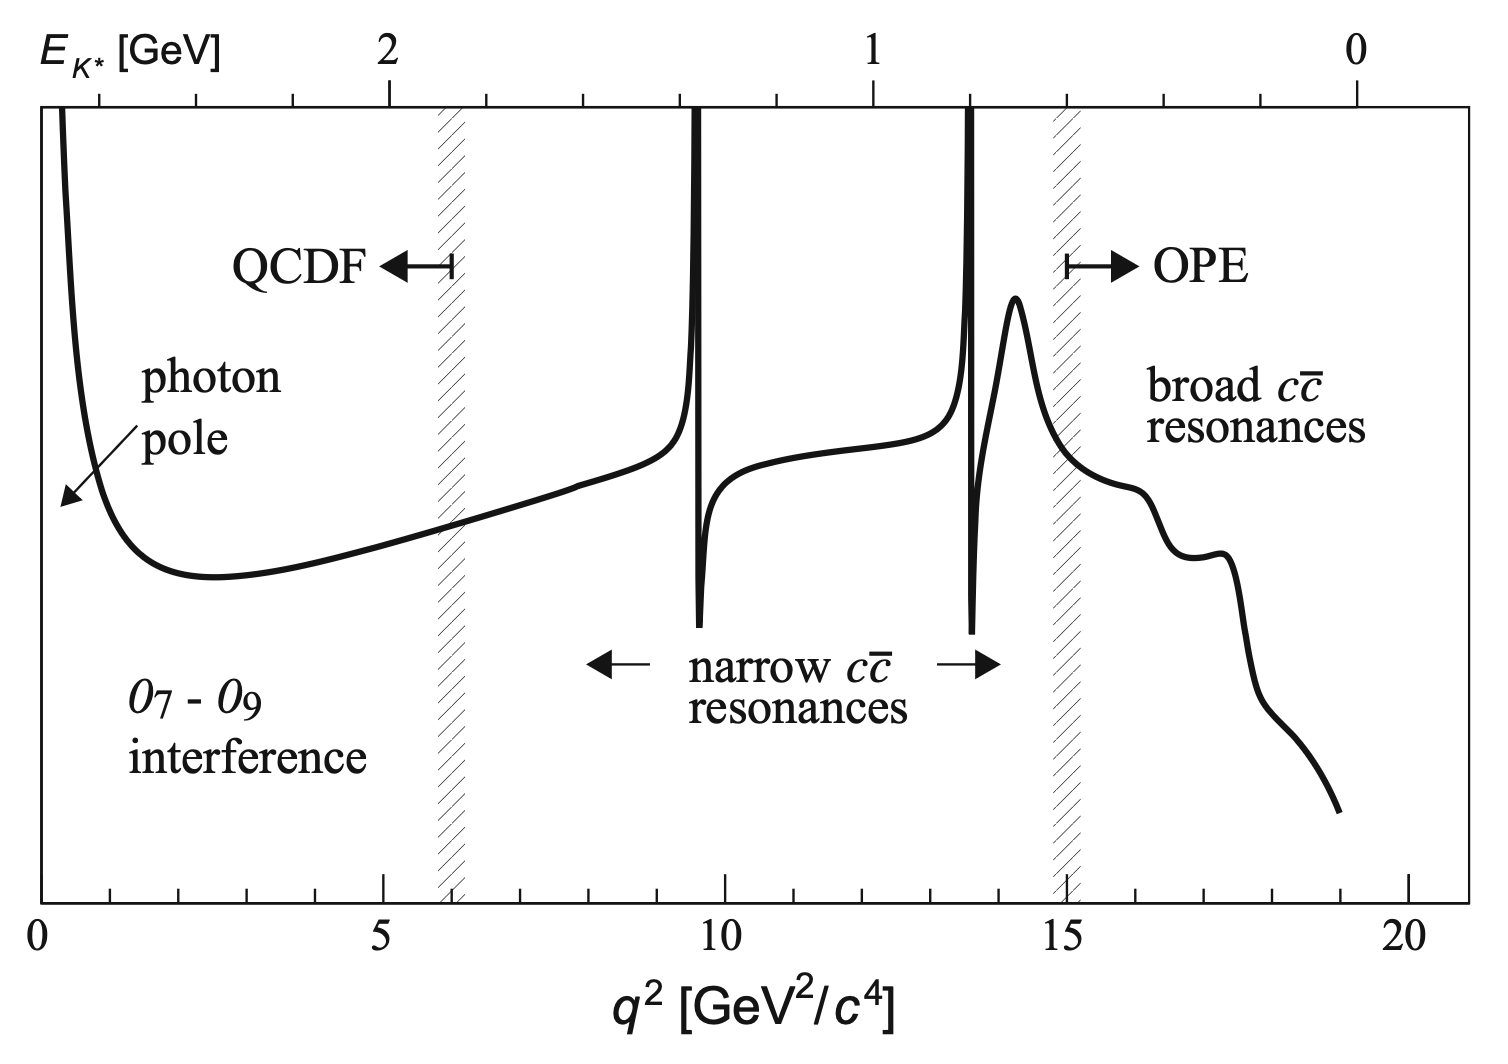
\includegraphics[width=0.9\textwidth]{figures/q2.png}
    \caption{A typical $q^2$ spectrum of the transition $b \to s \, l^+ \, l^-$, taken from \cite{blake2015}.}
    \label{fig:q2-spectrum}
\end{figure}

For low $q^2$, the spectrum is dominated by the photon pole originating from the decay $b \to s \, \gamma$, where the $\gamma$
further decays into a lepton pair. The central region is characterized by the narrow charmonium resonances $J/\psi$ and $\psi(2S)$,
each of which decays into a lepton pair. In the high $q^2$ region, above $\qty{15}{\giga\electronvolt\squared\per\lightspeed\tothe{4}}$,
the spectrum is dominated by the already mentioned penguin and $W$ boson box diagrams.
\chapter{The LHCb Experiment}
\label{ch:lhcb}

The Large Hadron Collider beauty (LHCb) experiment \cite{lhcb2008, lhcb2015} is one of the four main experiments at the Large Hadron Collider (LHC) \cite{lhc_machine2008} at the European Organization for Nuclear Research (CERN), which is located in Geneva, Switzerland. It is designed to study the properties of beauty and charm hadrons, with a primary focus on precision measurements of rare decays, CP violation, spectroscopy, and the search for NP.

At CERN, protons are accelerated to ultra-relativistic speeds through a complex of accelerators. The last stage in the acceleration chain is the LHC, a synchrotron particle collider situated $\qty{100}{\meter}$ underground, with a circumference of $\qty{26.7}{\kilo\meter}$. In the LHC, two proton beams are accelerated in opposite directions and made to collide at four interaction points, reaching a center-of-mass energy of $\sqrt{s} =  \qty{13}{\tera\electronvolt}$ during Run 2 and $\sqrt{s} = \qty{13.6}{\tera\electronvolt}$ in Run 3 of the LHC. Superconducting dipole magnets guide the particles around the ring, while quadrupole magnets focus them into tight beams. The acceleration is achieved using radio-frequency cavities.

The LHCb detector is located at the intersection point 8 of the LHC ring and is designed as a single-arm forward spectrometer, optimized for the predominantly forward and backward production of beauty and charm hadrons in $pp$ collisions. The following sections describe the LHCb detector in its Run 2 and Run 3 configurations, with a focus on the changes introduced by the upgrade for Run 3.

\section{Run 2}
\label{sec:lhcb_run2}
Run 2 of the LHC took place from 2015 to 2018. \cref{fig:lhcb_run2} shows a schematic overview of the LHCb detector during this data-taking period. The detector is composed of several subdetectors that can be grouped into two types of systems. The tracking system comprises the Vertex Locator (VELO), a dipole magnet, the Tracker Turicensis (TT), and three downstream tracking stations (T1, T2, and T3). The particle identification system includes the Ring Imaging Cherenkov (RICH) detectors, the electromagnetic and hadronic calorimeters (ECAL and HCAL), and the muon system (M1–M5). 
%The muon system additionally provides tracking information for muons.
\begin{figure}
    \centering
    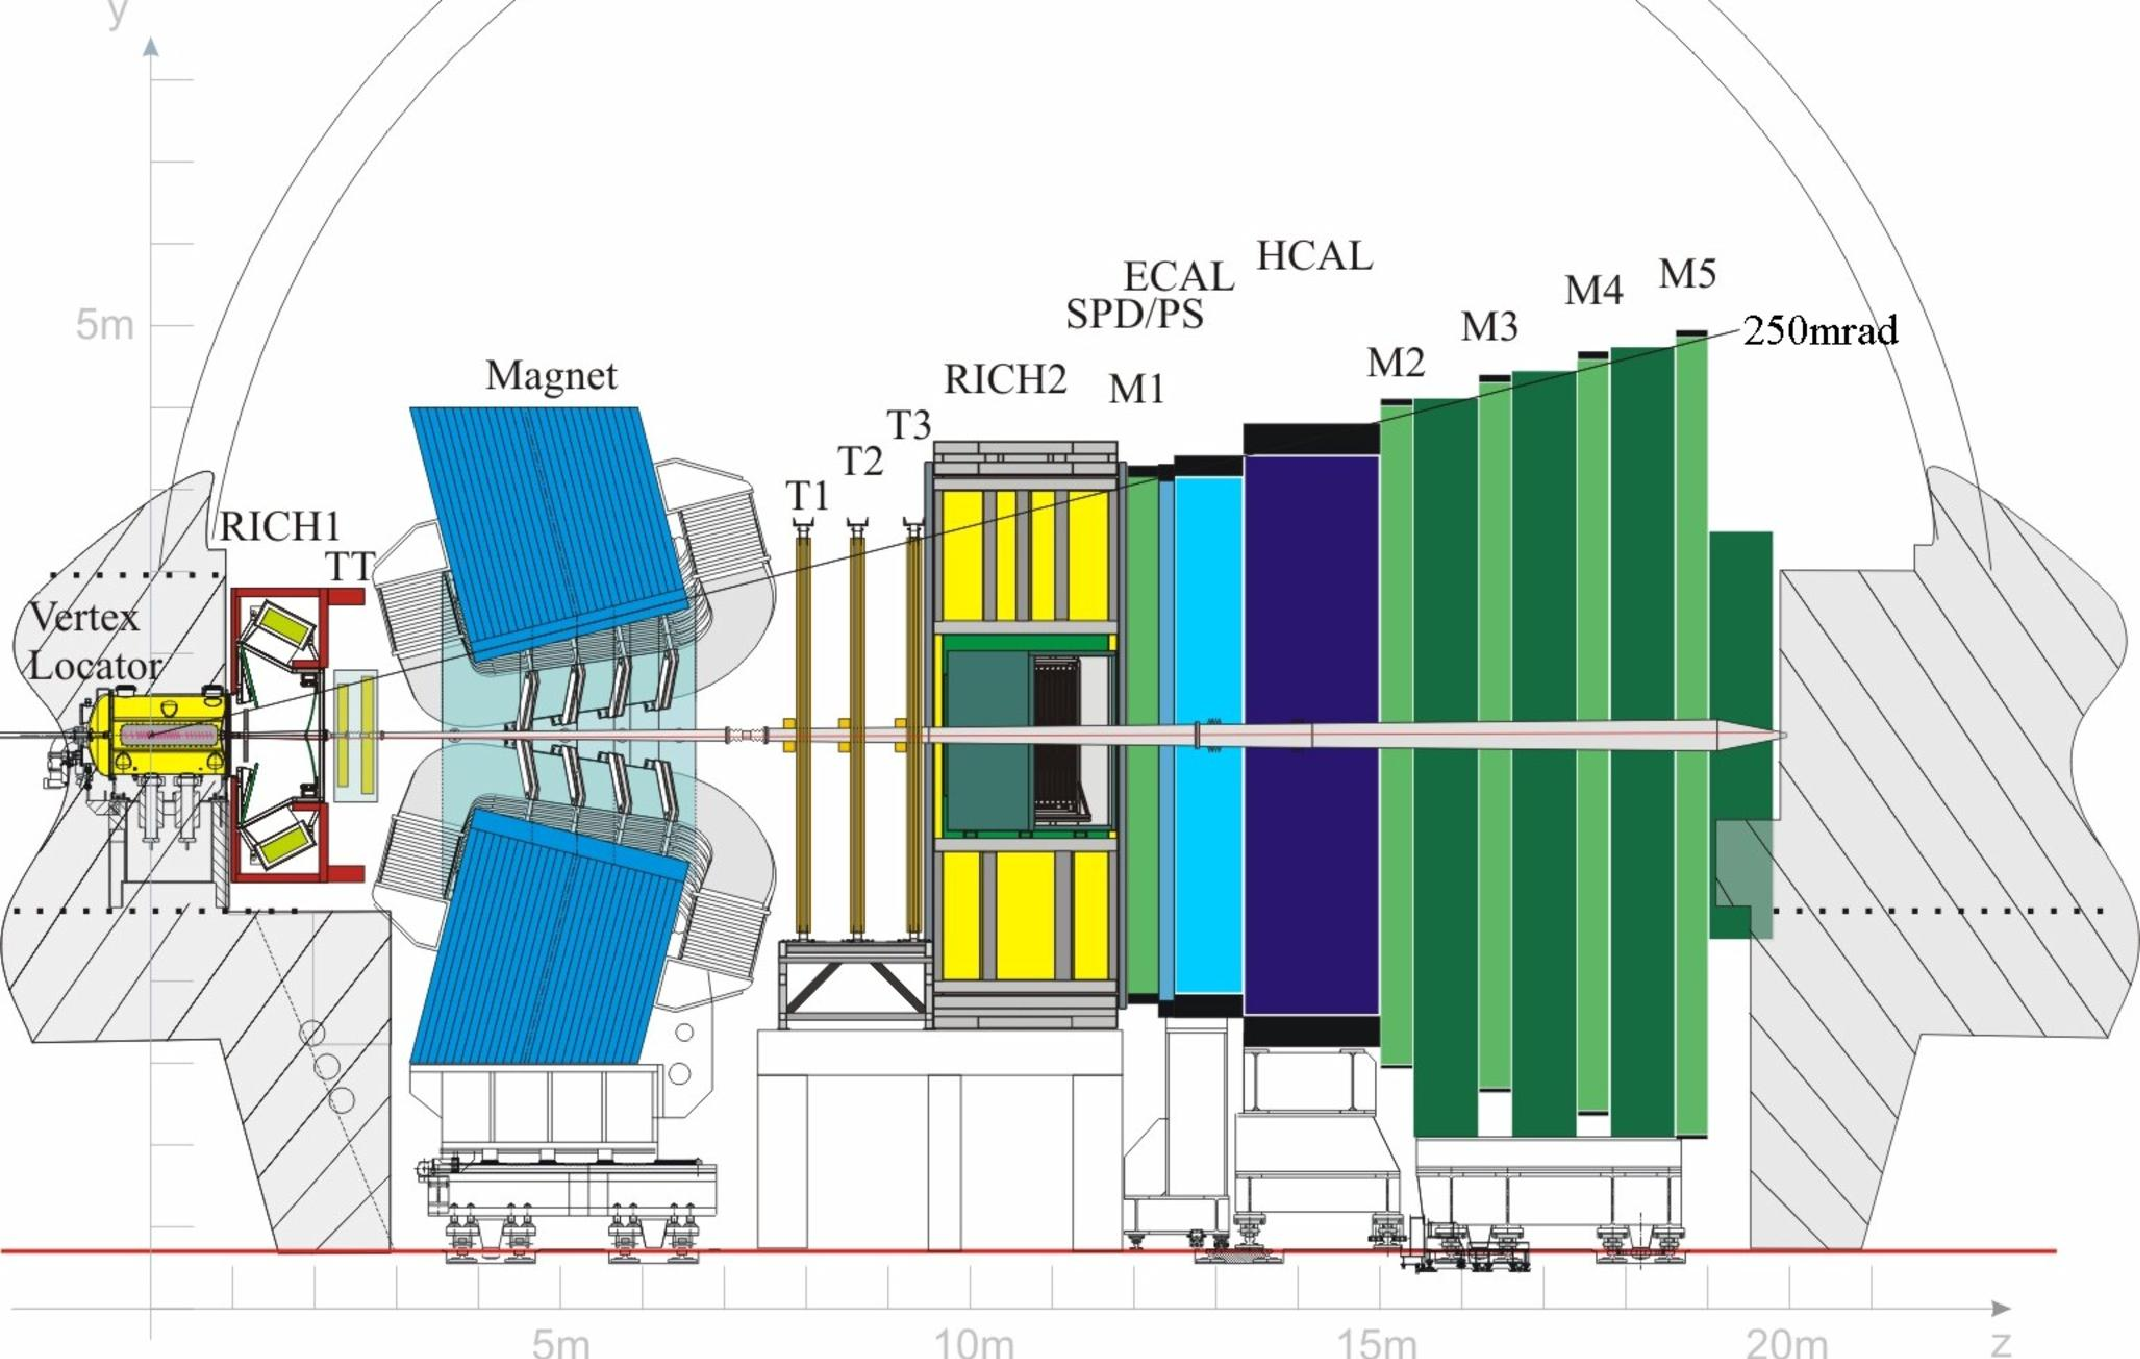
\includegraphics[width=0.9\textwidth]{figures/lhcb_run2.png}
    \caption{Side view of the LHCb detector and its subdetectors during Run 2, taken from \cite{calabrese2022_rich_run2}.}
    \label{fig:lhcb_run2}
\end{figure}

The VELO is a silicon microstrip detector that surrounds the $pp$ interaction region and is used to measure tracks of ionizing particles containing beauty or charm quarks as well as their primary and secondary vertices. The tracking stations and the TT are located behind the VELO and are essential for
the reconstruction of the trajectories of charged particles. T1, T2, and T3 each consist of a silicon microstrip Inner Tracker (IT) and an Outer Tracker (OT), a drift detector based on straw tube technology. The TT, also a silicon microstrip detector, is located between RICH1 and the magnet, whereas T1, T2, and T3 are positioned downstream of the magnet. This arrangement enables the measurement of charged-particle momenta via the bending of their trajectories in the magnetic field. Even in the absence of VELO information, the TT delivers upstream tracking data that is essential for the momentum reconstruction of long-lived particles such as the $\Lambda^0$ hyperon. In order to eliminate systematic effects, the magnet polarity is reversed several times during the year.

The RICH1 detector, located behind the VELO, and the RICH2 detector, located behind T3, are used for particle identification by measuring the Cherenkov radiation emitted by charged particles that travel faster than the speed of light in the detector medium. The angle $\Theta_{\text{c}}$ of the emitted Cherenkov radiation is dependent on the particle's velocity and the refractive index of the medium. The velocity can be expressed through the momentum $p$ and mass $m$ of the particle. This enables testing mass hypotheses using the reconstructed momentum and the measured Cherenkov angle. LHCb employs
two RICH detectors with different radiators to achieve particle identification across a wider momentum range.

The electromagnetic calorimeter (ECAL) and the hadronic calorimeter (HCAL) are located behind RICH2. They are used for energy reconstruction and particle identification. The ECAL intercepts electromagnetically interacting particles, mostly photons and electrons. These particles deposit their energy in the ECAL through electromagnetic showers, which can be used to reconstruct the particle's energy and impact position. The ECAL is made of alternating layers of lead and scintillating material, where the lead acts as an absorber material and the scintillating material as a sensitive medium to detect the electromagnetic showers. Since hadronic showers are larger in their longitudinal expansion than electromagnetic showers, the HCAL is placed behind the ECAL. It is made of iron and scintillating material, and works in a similar way to the ECAL, but is designed to measure the energy of hadrons, such as  pions and protons. In order to aid the particle identification process, the Scintillating Pad Detector (SPD) and Preshower Detector (PS) are placed in front of the ECAL. The SPD allows distinguishing between charged and neutral particles by measuring the scintillation light produced when charged particles pass through scintillator pads. Right behind the SPD, a thin lead converter is placed, followed by the PS. Photons and electrons start an early electromagnetic shower in the lead converter, which is then measured by scintillator pads in the PS, enabling the identification of these particles. 

The muon stations are the last elements of the LHCb detector. Muons are minimum ionizing particles and therefore pass through the calorimeters without losing large amounts of energy. A muon station consists of alternating layers of iron as an absorber and multi-wire proportional chambers, which are used to measure muon tracks. The absorber ensures that only muons reach the detector, enabling the identification of muons.

Within the constraints of the experiment’s technical and storage infrastructure, it is not feasible to record data at the full bunch-crossing rate of the LHC. Since many collisions produce background events of no interest, the LHCb detector employs several trigger systems to select events of potential relevance. The Level 0 trigger (L0) is a hardware trigger that selects events based on the information from the calorimeters and muon system, to filter events with high transverse momenta or energy above a defined threshold. The High Level Trigger (HLT) is the second trigger level and is fully software-based. It is further divided into HLT1, which uses partially reconstructed events, and HLT2, which uses fully reconstructed events, in order to perform the selection.

\section{Run 3}
\label{sec:lhcb_run3}
Run 3 of the LHC began in 2022 and is scheduled to continue until 2026. To enhance its performance and handle an instantaneous luminosity five times higher than in earlier runs, the LHCb detector underwent a major upgrade, referred to as Upgrade I \cite{lhcb_upgrade_I}. \cref{fig:lhcb_run3} presents a schematic overview of the detector following this Upgrade.
\begin{figure}
    \centering
    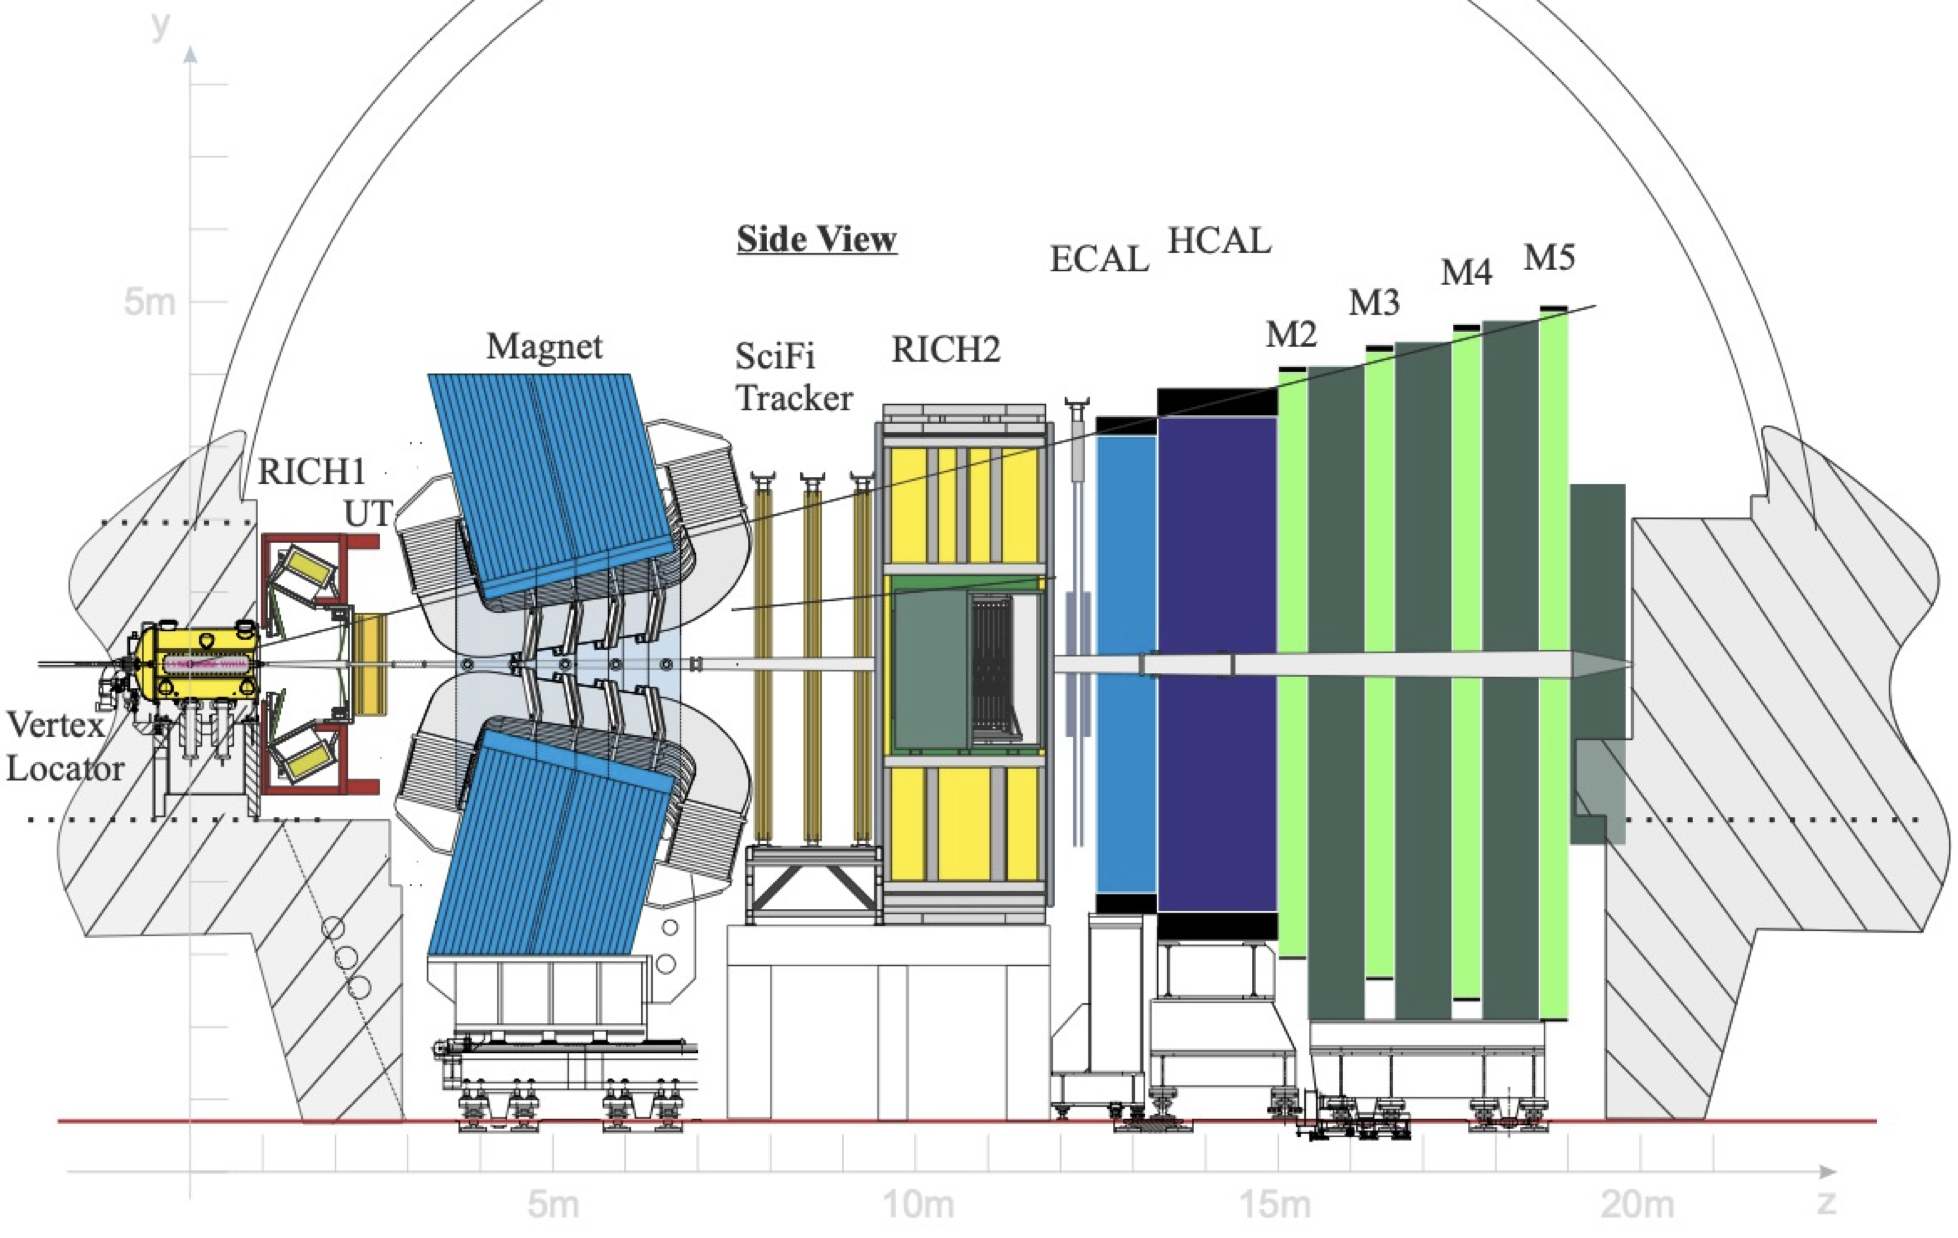
\includegraphics[width=0.9\textwidth]{figures/lhcb_run3.png}
    \caption{Side view of the LHCb detector and its subdetectors during Run 3, taken from \cite{lhcb_upgrade_I}.}
    \label{fig:lhcb_run3}
\end{figure}

Upgrade I introduced major changes to the LHCb experiment. The L0 trigger, which has been removed, lowered signal yields because its transverse energy and momentum thresholds led to the rejection of low-$p_{\text{T}}$, yet physically relevant, events.
The detector and trigger stages are therefore required to process the full crossing rate of $\qty{40}{\mega\hertz}$ provided by the LHC. This is achieved by upgrading the readout electronics, as well as optimizing the HLT algorithms and computing structures. Several subdetectors have been upgraded, removed, or replaced. The PS and SPD detectors, as well as the M1 muon station, were removed, as they were primarily used for the L0 trigger. The tracking system has been fully upgraded and now consists of a silicon-pixel VELO, the Upstream Tracker (UT), and the Scintillating Fiber Tracker (SciFi). The UT, a silicon-based detector, replaces the former TT station. The SciFi tracker comprises three stations, which supersede the previous T1, T2, and T3 stations. Each station contains four detection planes made of scintillating fiber mats, with varying fiber orientations. In addition, the photon detection systems of the RICH detectors have been upgraded.

\section{Impact of Upgrade I on Signal Yields}
\label{sec:lhcb_upgrade_effects}
Since this thesis measures the signal yield $N$ of the rare decay $\Lambda_b^0 \to \Lambda^0 \mu^+ \mu^-$ in both Run 2 and Run 3, it is important to discuss the effects of Upgrade I on this measure. The signal yield is given by
\begin{equation}
    N = 2 \, \mathcal{L} \, \epsilon \, \sigma_{b\bar{b}} \, f_{\Lambda_b^0} \, \mathcal{B}(\Lambda_b^0 \to \Lambda^0 \mu^+ \mu^-) \, \mathcal{B}(\Lambda^0 \to p \pi^-),
    \label{eq:signal_yield}
\end{equation}
where $\mathcal{L}$ is the integrated luminosity, $\sigma_{b\bar{b}}$ the production cross-section of beauty hadrons, $f_{\Lambda_b^0}$ the production fraction of the $\Lambda_b^0$ baryon, $\mathcal{B}$ denotes branching fractions, and $\epsilon$ the total efficiency. $\epsilon$ is the product of several components, including the detector acceptance and efficiencies from all stages of data processing from the trigger and reconstruction to the final signal selection. This analysis is CP-averaged, meaning that both the $\Lambda_b^0$ and $\bar{\Lambda}_b^0$ decays are included. This is reflected by the factor of 2 in \cref{eq:signal_yield}.

The first key difference concerns the total efficiency $\epsilon$, which is influenced by several changes introduced with Upgrade I. Enhancements to the trigger and detector systems affect both the trigger and reconstruction efficiencies, while modifications in the analysis strategy between Run 2 and Run 3 impact the selection efficiency. The second difference is the increased number of visible $pp$ interactions per bunch crossing $\mu$ in Run 3, which can lead to overlapping events and thereby affect the trigger and reconstruction performance. Furthermore, an increase in $\mu$ raises the instantaneous luminosity, yielding a higher integrated luminosity in a shorter time. 
\chapter{Run 2 Study}
\label{ch:run2}
In this chapter, the study performed on the Run 2 data is described in detail, which is based on an existing angular analysis \cite{Janina}. First, the data samples and Monte Carlo (MC) simulation used for the study are presented, followed by the online and offline selection criteria. The chapter then discusses the simulation corrections applied. A Multivariate Analysis (MVA) is performed to improve the signal purity, and finally, invariant mass fits are conducted to extract the signal yields.

\section{Data Samples}
\label{sec:run2_data_samples}
The $pp$ collision data samples analyzed in this study were recorded by the LHCb experiment between 2015 and 2018 during Run 2. The dataset corresponds to an integrated luminosity of $\mathcal{L} = \qty{6}{\femto\barn}^{-1}$ at a center-of-mass energy of $\sqrt{s} = \qty{13}{\tera\electronvolt}$. Several decay channels are of interest, particularly the rare decay $\Lambda_b^0 \to \Lambda^0 \mu^+ \mu^-$. In addition, the  resonant mode $\Lambda_b^0 \to \Lambda^0 J/\psi (\to \mu^+ \mu^-)$ is studied. It is used for the simulation calibration, as it has the same final-state particles but higher statistics due to the tree-level nature of the decay. The resonant mode is selected by applying the mass constraint $\vert m(J/\psi)-\qty{3096}{\mega\electronvolt} \vert < \qty{100}{\mega\electronvolt}$. Apart from this, the signal selection strategy follows that used in the rare decay mode.

The data is grouped into Long--Long (LL) and Downstream--Downstream (DD) categories, based on the track types of the decay products from $\Lambda^0 \to p \pi^-$. In this study, two types are considered: long and downstream tracks. For long tracks, particles leave hits in both the VELO and TT, providing tracking information upstream of the magnet. In contrast, downstream tracks do not produce hits in the VELO and are therefore reconstructed without this information. This occurs due to the relatively long lifetime of the neutral $\Lambda^0$ hyperon, which can decay outside the VELO acceptance. In this thesis, LL candidates refer to events where both the proton and the pion from the $\Lambda^0$ decay are reconstructed as long tracks, while DD candidates are events where both decay products are downstream tracks. Generally, downstream tracks are more challenging to reconstruct and exhibit poorer momentum resolution. Events with mixed track types are not considered in this thesis.
% as both particles originate from the same decay vertex and are expected to share the same track type.

In addition to the data, simulation samples are used. These samples are employed, among other purposes, to determine the signal shape in invariant mass fits, and to train Boosted Decision Trees (BDT) for the MVA. There is a simulation sample for each decay channel, year, and magnet polarity, reflecting the different conditions during data taking. The misidentification (misID) background component in the resonant mode, which is explained in \cref{sec:run2_selection}, is simulated as well.

\section{Online and Offline Selection}
\label{sec:run2_selection}
The study for the rare mode is conducted in the high-$q^2$ region above $\qty{15}{\giga\electronvolt\tothe{2}\per\lightspeed\tothe{4}}$, where penguin and $W$ boson box processes have a high statistic and narrow charmonium resonances are absent, as discussed in \cref{sec:q2-spectrum}. The $J/\psi$ samples are excluded from this cut.

There are multiple background sources present in the data. The online and offline selections are the first steps to remove this background. The most significant one is the combinatorial background, which is caused by the random combination of tracks in the detector. Another source is the misID background. This background originates from the misidentification of a $\pi^+$ as a proton in the decay $B^0 \to K^0_{\text{S}} J/\psi$, where the $K^0_{\text{S}}$ decays into $\pi^+$ and $\pi^-$. As a result, the $K^0_{\text{S}}$ mimics the decay products of the $\Lambda^0$ baryon. This background pollutes the signal region of the $J/\psi$ mode and is therefore accounted for in the analysis. Each selection step is applied to both the data and simulation samples for each decay channel.

\subsection{Online Selection}
\label{sec:run2_online_selection}
The online event selection is performed by the LHCb trigger system, as described in \cref{sec:lhcb_run2}, and serves to reduce the data volume that must be stored during data taking. The L0 trigger selects events containing one or two muons with high transverse momentum. HLT1 and HLT2 then identify events with high-quality tracks and decay topologies characteristic of the rare decay. All trigger lines used in this analysis are Trigger On Signal (TOS), meaning the decision is based on the signal decay products. Trigger Independent of Signal (TIS) lines are not used in this study. A summary of the trigger decisions is shown in the appendix. Prior to tuple creation, further data reduction and signal selection are performed centrally in the LHCb data flow through stripping. Here, the stripping line \texttt{Bu2LLk\_mmLine} is employed.
%\textcolor{red}{Hier muss noch die stripping line hin:  inclusive stripping line Bu2LLK_mmLine}

\subsection{Offline Selection}
\label{sec:run2_offline_selection}
Following the online selection, the offline selection is subsequently applied to the preselected events. It is adopted from the angular analysis \cite{Janina} and has already been optimized. The offline selection criteria are summarized in \cref{tab:run2_offline_selection}.
\begin{table}
    \centering
    \sisetup{table-format=2.2}
    \caption{Offline selection cuts used in the Run 2 study.}
    \label{tab:run2_offline_selection}
    \begin{tblr}{
        colspec = {c c},
    }
        \toprule
        Particle & Cuts\\
        \midrule
        $\mu^+$, $\mu^-$ & \texttt{hasMuon}\,, \quad \texttt{hasRich}\,, \quad \texttt{inAccMuon}\\
                         & $p_T > \qty{800}{\mega\electronvolt}$\,, \quad $p > \qty{3000}{\mega\electronvolt}$ \\
                         & \texttt{ProbNNMu} > 0.1 \\
        \cline{1-2}
        $\Lambda^0$      & $\vert m - \qty{1116}{\mega\electronvolt} \vert < \qty{8}{\mega\electronvolt}$\,, \quad $0 < \tau < \qty{2}{\pico\second}$ \\
                         & $\Theta_{\text{DIRA}} > 0$\,, \quad $\chi^2_\text{FD} > 0$ \\
                         & $0 < z_\text{EV} < \qty{2320}{\milli\meter}$ \\
        \cline{1-2}
        $\Lambda_b^0$    & $\chi^2_{DTF} / \text{ndof}$ > 0 \\
        \bottomrule
    \end{tblr}
\end{table}

Fiducial cuts select events from a well-defined phase space for the detector. These cuts include requiring the muon tracks to lie within the muon system acceptance (\texttt{inAccMuon}), applying momentum thresholds for the muons, and selecting on the $z$ coordinate of the $\Lambda^0$ end vertex. The remaining muon selection criteria ensure robust muon identification by requiring hits in the muon stations and information from the RICH detectors, while rejecting candidates with a low probability of being a muon as estimated by a neural network. The properties of the $\Lambda^0$ can be determined reliably. Especially for LL events, its long flight distance and well-tracked decay products provide clear spatial and kinematic information, allowing for an effective selection based on its reconstructed properties. Finally, the $\chi^2_{DTF}$ value of the $\Lambda_b^0$ is required to be positive, since a failed Decay Tree Fitter (DTF) fit yields negative values. 
 
Truth matching is applied to the simulation samples to ensure only correctly reconstructed signal events are considered. Two methods are used in this thesis. The first matches each reconstructed particle and its mother to their generator-level counterparts using the TRUEID and MOTHERID, which are identifiers that follow the MC particle numbering convention of the Particle Data Group \cite{pdg2024}. The second method uses the \textit{BKGCAT} tool \cite{LHCbBKGCAT}, which classifies each candidate as either signal or a specific background type. Candidates from the rare and $J/\psi$ mode are selected from those \textit{BKGCAT} categories whose $\Lambda_b^0$ mass distributions exhibit a characteristic signal shape \footnote{Rare mode events are accepted if $\texttt{BKGCAT} = 10$ (quasi-signal) or $50$ (low-mass background) and $J/\psi$ mode events if $\texttt{BKGCAT} = 0$ (signal) or $50$.}.  The misID events, on the other hand, are selected with the first method \footnote{The misID truth matching requiers $\vert \texttt{TRUEID}_{\Lambda^0} \vert = 310$, $\vert \texttt{TRUEID}_{\Lambda_b^0} \vert = 511$, $\vert \texttt{MOTHERID}_{\Lambda^0} \vert = 511$,  and $\vert \texttt{MOTHERID}_{J/\psi} \vert = 511$. In this notation, 511 and 310 denote the $\Lambda_b^0$ and $\Lambda^0$ baryons, respectively.}.


\section{Simulation Corrections}
\label{sec:run2_mc_corrections}
Exact reproduction of the data by simulations is not feasible, owing to the complexity of the measurement, including physics modeling, detector effects, and real-world operational variations. However, known modeling inaccuracies can be corrected, as outlined in this section. In the absence of a dedicated calibration dataset, a representative decay mode is required to describe the measured signal. The $J/\psi$ decay is employed for this purpose, as it provides high statistics and involves the same final-state particles as the rare mode. Fits to the invariant mass distribution of the $\Lambda_b^0$ are performed on the $J/\psi$ mode data with the rare mode online and offline selection applied \footnote{The fits are shown in the appendix}. From these fits, sWeights are computed and subsequently used to construct a representative signal proxy.
%The simulations employed in this study do not exactly reproduce the data, owing to the high complexity of the detector and physics processes. However, many sources of discrepancies can be corrected. This section outlines the corrections applied to the simulation samples to ensure that they accurately represent the observed data. The $J/\psi$ decay mode is used for calibration in the absence of a dedicated independent dataset, as it provides higher statistics than the rare decay mode while involving the same final-state particles. For this purpose, sWeighted data are obtained from invariant mass fits to the $\Lambda_b^0$ mass distribution in the $J/\psi$ mode. The fits are shown in the appendix.

\subsection{L0 Trigger Corrections}
\label{sec:run2_trigger_corrections}
The efficiency of the L0 trigger is dependent on the kinematic properties of the muons, such as their transverse momentum and pseudorapidity. To account for this, the simulation is reweighted to match the L0 trigger efficiency in sWeighted data. The efficiencies needed for the computation of the weight maps are calculated using the \textit{TISTOS} method \cite{TISTOS} on a dedicated $B^+ \to J/\psi \,K^+$ calibration sample. This correction is done separately for the \texttt{Muon} and \texttt{DiMuon} trigger decisions. The final L0 trigger weight $w_\text{L0}$ is then computed as
\begin{equation*}
    w_{\text{L0}} = 1 - (1- \texttt{Muon} \cdot w_{\text{Muon}})(1- \texttt{DiMuon} \cdot w_{\text{DiMuon}}),
\end{equation*}
where $w_{\text{Muon}}$ and $w_{\text{DiMuon}}$ are the weights for the \texttt{Muon} and \texttt{DiMuon} trigger decisions, respectively.

\subsection{Lifetime Correction}
\label{sec:run2_lifetime_correction}
 A correction is applied to adjust for the difference between the fixed mean lifetime used in the simulation and the updated measurements of the $\Lambda_b^0$ baryon lifetime \cite{pdg2024}. A weight $w_{\tau}$ is computed for each event in the simulation samples as
\begin{equation*}
    w_{\tau} = \frac{\exp \left(-\frac{t}{\tau_{\text{new}}}\right)}{\exp \left(-\frac{t}{\tau_{\text{old}}}\right)},
\end{equation*}
where $t$ is the measured lifetime, $\tau_{\text{old}} = \qty{1.451}{\pico\second}$ the mean lifetime used in the simulation, and $\tau_{\text{new}} = \qty{1.468}{\pico\second}$ \cite{pdg2024} the updated lifetime. The effect of the lifetime correction on the lifetime distribution of the $\Lambda_b^0$ in the $J/\psi$ channel is shown in the appendix.

\subsection{Kinematic Correction}
\label{sec:run2_kinematic_corrections}
The kinematic properties of $b$-hadrons are known to be mismodeled in the LHCb simulations. This can be corrected by reweighting the simulation samples using a weight map segmented into bins of $p_{\text{T}}$ and $\eta$. The weight map is calculated with the $J/\psi$ simulation and sWeighted data distributions. As shown in the appendix, this kinematic correction effectively adjusts the transverse momentum distributions.
%\begin{figure}
%   \centering
%    \begin{subfigure}[b]{0.48\textwidth}
%        \centering
%        \includegraphics[width=\textwidth]{../plots/MC_Data_agreement/R2/ll/Lambdab_log10_pT.pdf}
%        \caption{LL}
%    \end{subfigure}
%    \hfill
%    \begin{subfigure}[b]{0.48\textwidth}
%        \centering
%        \includegraphics[width=\textwidth]{../plots/MC_Data_agreement/R2/dd/Lambdab_log10_pT.pdf}
%        \caption{DD}
%    \end{subfigure}
%    \caption{The $\log_{10}(p_{\text{T}})$ distributions of the $\Lambda_b^0$ baryon for the LL and DD categories in the $J/\psi$ mode, shown before %(blue) and after (red) the correction, and compared with sWeighted data (black).}
%    \label{fig:run2_kinematic_corrections}
%\end{figure}

\subsection{Particle Identification Correction}
\label{sec:run2_pid_correction}
The feature \texttt{ProbNNMu}, which represents the probability of a particle being a muon, is used in the offline selection. It was not calibrated in the previous angular analysis \cite{Janina}, but needs to be calibrated using the \textit{PIDGen2} tool \cite{pidgen2}, which is designed to correct the particle identification (PID) response in simulation. Here, the transformation method of the \textit{PIDGen2} tool is used, which employs $p_{\text{T}}$, $\eta$, and the event multiplicity nTracks as the input features. The nTracks feature is mismodeled as well, but can be shifted by multiplying each nTracks value by a constant factor of $1.1$ to accurately represent the distribution seen in sWeighted data. The calibration uses a dedicated $J/\psi \to \mu^+ \mu^-$  calibration sample for each year and magnet polarity. The corrected \texttt{ProbNNMu} feature of the rare mode simulation is shown in the appendix.
%\begin{figure}
%    \centering
%    \includegraphics[width=0.48\textwidth]{../plots/pid_correction/ProbNNmu_comparison.pdf}
%    \caption{The \texttt{ProbNNMu} distribution of the rare mode simulation for the LL and DD categories combined,
%    shown before (blue) and after (red) the PID correction, compared with the $J/\psi$ sWeighted data (black).}
 %   \label{fig:run2_pid_correction}
%\end{figure}

\section{Multivariate Analysis}
\label{sec:run2_mva}
The fully-calibrated simulation samples are employed to train BDTs, with the aim of separating signal events from combinatorial background and minimizing its presence in the dataset. A BDT is a supervised machine learning algorithm that sequentially combines multiple decision trees, where each tree classifies events by making a series of binary decisions based on its input variables and corrects the misclassifications of the previous trees. Separate BDTs are trained for the LL and DD categories. Both the training and the overtraining checks are performed using the \textit{TMVA} package within \textit{ROOT} \cite{root}. The calibrated rare mode simulation is used as the signal proxy for the training. The mass sidebands, $ \qty{5000}{\mega\electronvolt} < m(\Lambda_b^0) < \qty{5400}{\mega\electronvolt}$ and $\qty{5720}{\mega\electronvolt} < m(\Lambda_b^0) < \qty{6500}{\mega\electronvolt}$, are used as a proxy for the background, as they are well separated from the signal peak. The BDT input features were selected based on their ability to distinguish signal from background, as determined by examining their distributions. The BDT was then trained iteratively, removing features with high correlation or low importance to achieve a stable and well-performing classifier. A list of these features, ordered by their feature importance, is shown in the appendix.  The BDT cut value is optimized using the Punzi Figure of Merit (FOM) \cite{punzi}, defined as
\begin{equation*}
    \text{FOM}_{\text{Punzi}} = \frac{\epsilon_{\text{S}}}{a/2 + \sqrt{B}},
\end{equation*}
where $\epsilon_{\text{S}}$ denotes the signal efficiency determined on simulation, $B$ the number of background events passing the BDT selection for a given cut, and $a$ denotes the desired statistical significance, which is chosen to be $a=5$ for a $5\sigma$ discovery. $B$ is determined by fitting the selected data and calculating the background yield within a $3 \,\sigma$ region around the signal peak. The Punzi FOM is maximized to determine the optimal cut value. It is well-suited for rare decay searches, as it relies on the signal efficiency rather than the absolute signal yield, making it more robust when the expected signal count is small or inaccessible in a blinded analysis. Since plateaus are observed near the maxima \footnote{This behavior is observed for all BDTs in both runs. Therefore, a more relaxed cut is adopted throughout. As an example, the Punzi FOM for the Run 2 LL and Run 3 DD BDT is shown in the appendix.}, a looser cut is chosen in order to increase the statistics for the mass fits.
The main characteristics and performance metrics of the two BDTs are given in \cref{tab:run2_mva_summary}.
\begin{table}
    \centering
    \caption{Characteristics and performance metrics of the Run 2 BDTs.}
    \label{tab:run2_mva_summary}
    \sisetup{table-format=2.2}
    \begin{tblr}{
        colspec = {c c c c c c c},
        column{1} = {c},
    }
        \toprule
         & Trees & Depth & Learning Rate & ROC Score & Cut Value \\ 
        \midrule
        LL & $180$ & $4$ & $0.12$ & $0.985$ & $0.9$\\
        DD & $200$ & $4$ & $0.10$ & $0.972$ & $0.9$\\
        \bottomrule
    \end{tblr}
\end{table}

\section{Invariant Mass Fits}
\label{sec:run2_mass_fits}
Following the selection, the signal yields are extracted from the invariant mass distributions of the $\Lambda_b^0$ baryon using a maximum likelihood fit performed with the \textit{RooFit} toolkit \cite{roofit}. The signal component is described by the linear sum of two double-sided Crystal Ball functions. On the other hand, the combinatorial background is modeled by an exponential function. A fit to the simulated signal is conducted to determine the unknown signal shape. In the data fits, only the mean, yield, and width of the signal are left free, while the tail parameters are fixed to the values obtained from the fits to the simulation. \cref{fig:run2_mass_fits} shows the invariant mass fits for LL and DD candidates in the rare decay mode.
\begin{figure}
    \centering
    \begin{subfigure}[b]{0.48\textwidth}
        \centering
        \includegraphics[width=\textwidth]{../plots/mass_fits/RM_dd_channel_data.pdf}
        \caption{DD}
    \end{subfigure}
    \hfill
    \begin{subfigure}[b]{0.48\textwidth}
        \centering
        \includegraphics[width=\textwidth]{../plots/mass_fits/RM_ll_channel_data.pdf}
        \caption{LL}
    \end{subfigure}
    \caption{Fits to the invariant mass distribution of the $\Lambda_b^0$ baryon with the full rare mode selection applied, shown for DD (right) and LL (left) events.}
    \label{fig:run2_mass_fits}
\end{figure}

The signal yields obtained from the mass fits are $N = \num{409(23)}$ for the DD and $N = \num{297(19)}$ for the LL category. The DD category is more frequent than the LL category, owing to the relatively long lifetime of the $\Lambda^0$ hyperon.
\chapter{Run 3 Study}
\label{ch:run3}
This chapter presents the first study of the rare decay $\Lambda_b^0 \to \Lambda^0 \mu^+\mu^-$ with data from Run 3 of the LHC. The analysis strategy from Run 2, as outlined in \cref{ch:run2}, is adopted here, except that the simulation correction is omitted. In the following chapter, the key findings of the Run 3 study are presented and compared to the findings of the Run 2 study.


\section{Data Samples}
\label{sec:run3_data_samples}
The data used in this study were collected in 2024 by the LHCb experiment during Run 3 of the LHC. They are organized into blocks, each corresponding to specific data-taking conditions, such as magnet polarity. This study uses blocks five to eight, which correspond to the last weeks of 2024 data taking, during which the subdetectors had mostly finished their commissioning. The data samples correspond to an integrated luminosity of $\qty{3.33}{\femto\barn}^{-1}$ at a center-of-mass energy of $\qty{13.6}{\tera\electronvolt}$.

For each block, simulation is used for both the rare decay and the $J/\psi$ mode. No Run 3 simulation samples are available for the misID background of the $J/\psi$ mode, instead, $B^0 \to K^0_{\text{S}} J/\psi$ simulations from Run 2 are used for the $J/\psi$ mass fit.

As in the Run 2 study, events are classified into LL and DD categories, depending on whether the decay products of the $\Lambda^0$ baryon left hits in the VELO or not.

\section{Online and Offline Selection}
\label{sec:run3_selection}
The offline selection follows the procedure used in Run 2, as discussed in \cref{sec:run2_selection}. The selection criteria are listed in \cref{tab:run2_offline_selection}, with the exception of the variable $\chi^2_{\text{FD}}$, which is absent in the Run 3 simulation samples and therefore not included in the offline selection. 

Following the Upgrade I implementation of a new trigger system, the online selection has been modified. In Run 3, two dedicated HLT2 trigger lines, namely \texttt{Hlt2RD\_LbToLMuMu\_LL} and \texttt{Hlt2RD\_LbToLMuMu\_DD}, are employed for the LL and DD selection, effectively replacing the stripping procedure used in previous runs. In contrast, the HLT1 selection remains unchanged.

\section{Multivariate Analysis}
\label{sec:run3_mva}
The MVA strategy outlined in \cref{sec:run2_mva} is also employed in the Run 3 analysis. However, the simulation samples are uncalibrated, and several input features available in Run 2 are absent in Run 3. The BDT features, ranked by their importance, are listed in the appendix, while \cref{tab:run3_mva_summary} summarizes the BDT characteristics and performance metrics.
\begin{table}
    \centering
    \caption{Characteristics and performance metrics of the Run 3 BDTs. The cut value is determined using the same procedure as in Run 2.}
    \label{tab:run3_mva_summary}
    \sisetup{table-format=2.2}
    \begin{tblr}{
        colspec = {c c c c c c c},
        column{1} = {c},
    }
        \toprule
         & Trees & Depth & Learning Rate & ROC Score & Cut Value \\ 
        \midrule
        LL & $160$ & $3$ & $0.10$ & $0.979$ & $0.9$\\
        DD & $170$ & $3$ & $0.12$ & $0.989$ & $0.9$\\
        \bottomrule
    \end{tblr}
\end{table}

To assess the quality of the uncalibrated Run 3 simulation, the distribution of $\log_{10}(p_{\text{T}}(\Lambda_b^0))$ for DD events is compared between the Run 3 simulation, the Run 2 simulation, and the sWeighted data in the $J/\psi$ mode in Run 3. Variables that were well-modeled in Run 2 also show good agreement with the sWeighted data in Run 3, whereas $p_{\text{T}}(\Lambda_b^0)$ is known to be mismodeled in the initial Run 2 simulation, as discussed in \cref{sec:run2_kinematic_corrections}. This motivates the comparison presented in \cref{fig:run3_feature_check}.
\begin{figure}
    \centering
    \begin{subfigure}[b]{0.48\textwidth}
        \centering
        \includegraphics[width=\textwidth]{../plots/Run2_Run3_comparison/dd/log10_Lambdab_pT.pdf}
        \caption{Comparison between the Run 2 calibrated (red) and uncalibrated (blue) simulation with the Run 3 simulation (black) for the DD category.}
    \end{subfigure}
    \hfill
    \begin{subfigure}[b]{0.48\textwidth}
        \centering
        \includegraphics[width=\textwidth]{../plots/MC_Data_agreement/R3/dd/log10_Lambdab_pT.pdf}
        \caption{Comparison between the Run 3 simulation (red) and sWeighted data (black) for the DD category.}
    \end{subfigure}
    
    \caption{Comparison plots of the feature $\log_{10}(p_{\text{T}}(\Lambda_b^0))$ for the DD category. All plots are created using the $J/\psi$ mode.}
    \label{fig:run3_feature_check}
\end{figure}

The uncalibrated Run 2 and Run 3 simulations exhibit similar distributions. In Run 2, the application of the kinematic correction shifts the distribution toward lower momenta, corresponding to the direction in which the Run 3 sWeighted data deviate relative to the Run 3 simulation. The comparison indicates that $p_{\text{T}}(\Lambda_b^0)$ remains mismodeled in the Run 3 simulation.

The ROC score for the LL BDT is slightly worse compared to Run 2, whereas the DD BDT shows an improvement. The factors influencing the BDT performance include the non-optimized preselection in Run 3, which determines the initial signal-to-background distribution, the absence of simulation calibration, which is suboptimal for performance, and additional effects arising from the BDT tuning itself.

\section{Invariant Mass Fits}
\label{sec:run3_mass_fits}
Following the offline, online, and BDT selections, fits to the invariant mass distributions of the $\Lambda_b^0$ baryon in the rare decay mode are performed as described in \cref{sec:run2_mass_fits}. The same selection strategy is applied to the $J/\psi$ mode, for which corresponding fits are also carried out. In the $J/\psi$ mode, the signal and combinatorial background are modeled in the same way as in the rare decay mode, while the misID background is described using a double-sided Crystal Ball function. The tail parameters for the signal and misID component are determined by fits on simulation. The mass fits are shown in \cref{fig:run3_mass_fits_combined}.
\begin{figure}[htbp]
    \centering
    % Rare decay mode
    \begin{subfigure}[b]{0.48\textwidth}
        \centering
        \includegraphics[width=\textwidth]{../plots/mass_fits/R3/RM_dd_channel_data.pdf}
        \caption{Rare mode, DD}
    \end{subfigure}
    \hfill
    \begin{subfigure}[b]{0.48\textwidth}
        \centering
        \includegraphics[width=\textwidth]{../plots/mass_fits/R3/RM_ll_channel_data.pdf}
        \caption{Rare mode, LL}
    \end{subfigure}
    
    % J/psi mode
    \begin{subfigure}[b]{0.48\textwidth}
        \centering
        \includegraphics[width=\textwidth]{../plots/mass_fits/R3/Jpsi_channel_BDTG_data_dd.pdf}
        \caption{$J/\psi$ mode, DD}
    \end{subfigure}
    \hfill
    \begin{subfigure}[b]{0.48\textwidth}
        \centering
        \includegraphics[width=\textwidth]{../plots/mass_fits/R3/Jpsi_channel_BDTG_data_ll.pdf}
        \caption{$J/\psi$ mode, LL}
    \end{subfigure}

    \caption{Fits to the invariant mass distribution of the $\Lambda_b^0$ baryon with the full rare mode selection applied, shown for DD (right) and LL (left) candidates in the rare (top) and $J/\psi$ mode (bottom).}
    \label{fig:run3_mass_fits_combined}
\end{figure}

The signal yields obtained from the rare mode mass fits are $N = \num{99(11)}$ for the DD and $N = \num{132(13)}$ for the LL category. For the $J/\psi$ mode, the yields amount to $N = \num{3212(60)}$ for DD and $N = \num{5297(75)}$ for LL.

\section{Signal Yield Comparison}
\label{sec:run3_yield_comparison}
\cref{sec:lhcb_upgrade_effects} describes the detector and trigger modifications introduced by Upgrade I that have the potential to influence the signal yield of the rare baryonic decay under investigation. The integrated luminosities differ between the two runs. Therefore, the Run 2 yield is scaled by the factor $\mathcal{L}_{\text{Run 3}}/\mathcal{L}_{\text{Run 2}}$ to allow for a meaningful comparison. \cref{tab:yield_comparison} shows an overview of the yields for both runs, as well as the scaled yields.
\begin{table}
    \centering
    \caption{Comparison of the signal yields for the rare decay $\Lambda_b^0 \to \Lambda^0 \mu^+ \mu^-$ in Run 2 and Run 3. The Run 2 yields are additionally scaled by the factor $\mathcal{L}_{\text{Run 3}}/\mathcal{L}_{\text{Run 2}}$.}
    \label{tab:yield_comparison}
    \sisetup{table-format=2.2}
    \begin{tblr}{
        colspec = {c S S S S},
        row{1} = {guard, mode = math}
    }
        \toprule
        & N_{\text{Run 2}} & N_{\text{Run 3}} & N_{\text{Run 2, scaled}} & \frac{N_{\text{Run 2, scaled}} - N_{\text{Run 3}}}{N_{\text{Run 2, scaled}}} \\ 
        \midrule
        LL & \num{297(19)} & \num{132(13)} & \num{165(10)} & \qty{20(9)}{\percent}\\
        DD & \num{409(23)} & \num{99(11)}  & \num{227(13)} & \qty{56(5)}{\percent}\\
        \bottomrule
    \end{tblr}
\end{table}

Several caveats must be considered when interpreting the reduction in signal yield in Run 3. First, the simulation used in Run 3 lacks calibration, which is suboptimal for the MVA, as the BDTs are trained on simulation samples intended to represent the signal. It is reasonable to expect that the BDT performance would improve with well-calibrated simulation samples, leading to higher signal efficiency, reduced background contamination, and consequently increased yields. Furthermore, the offline selection employed in this study remains unchanged from Run 2, with the $\chi^2_{\text{FD}}$ cut omitted. Optimizing the offline selection in Run 3 would not only improve its performance but could also benefit the BDT. It is noteworthy that the reduction in yield is more pronounced for the DD category. This can be understood in the context of \cref{eq:signal_yield}, where the integrated luminosity $\mathcal{L}$ and total efficiency $\epsilon$ vary between the two runs. While the effect of the integrated luminosity has been accounted for, variations in the total efficiency also influence the yield. The total efficiency accounts for all stages of the measurement process, including detector acceptance, trigger and reconstruction efficiencies, as well as the efficiencies associated with the analysis selection. This is particularly relevant for the DD candidates, as the new UT was still in the installation and commissioning phase during the Run 3 data-taking period used in this study. The UT plays a crucial role for DD events, providing tracking information upstream of the magnet that is needed for momentum reconstruction. In contrast, LL events are less affected by the UT, as their reconstruction benefits from VELO information.

As a cross-check, the $J/\psi$ yields are also considered. The signal-yield ratio of LL-to-DD events is compared between Run 2 and Run 3 for both the rare and $J/\psi$ modes. Owing to the similarity of the two modes, the LL-to-DD ratios are expected to exhibit a comparable trend within each run. Since both Run 3 modes follow the same suboptimal selection procedure, they are subject to identical limitations inherent to the selection. The ratios are summarized in \cref{tab:ratios}.
\begin{table}
    \centering
    \caption{Comparison of the signal-yield ratios of LL-to-DD events observed in the Run 2 and Run 3 rare and $J/\psi$ modes. The fits for the Run 2 $J/\psi$ mode used to determine the signal yields are shown in the appendix. They were conducted analogously to the Run 3 $J/\psi$ mass fits, as described in \cref{sec:run3_mass_fits}.}
    \label{tab:ratios}
    \sisetup{table-format=2.2}
    \begin{tblr}{
        colspec = {S S S S S},
    }
        \toprule
        & \SetCell[c=2]{c}{{{Rare Mode}}} && \SetCell[c=2]{c} {{{$J/\psi$ Mode}}} & \\
        \cmidrule[lr]{2-3} \cmidrule[lr]{4-5}
        & \text{Run 2} & \text{Run 3} & \text{Run 2} & \text{Run 3} \\
        \midrule
        $\frac{N_{\text{LL}}}{N_{\text{DD}}}$ 
        & \num{0.73(0.06)} 
        & \num{1.33(0.20)} 
        & \num{0.776(0.009)} 
        & \num{1.65(0.04)} \\
        \bottomrule
    \end{tblr}
\end{table}

In Run 3, both the rare and $J/\psi$ modes exhibit a lower fraction of DD events relative to LL events, whereas in Run 2, the opposite trend was observed. This pattern is consistent with the hypothesis that the UT status during the considered data-taking period adversely affects DD signal reconstruction.

\section{Future Improvements}
\label{sec:run3_future_improvements}
The presented studies remain open to further improvement, starting with the implementation of an optimized offline selection and the calibration of the simulation. As discussed in \cref{sec:run3_yield_comparison}, implementing these improvements could increase the measured yields in Run 3. Moreover, calibrated simulations would enable a more accurate evaluation of how well the simulation represents the data. To verify whether the yield reduction in Run 3 is not solely caused by the non-optimized selection, the total selection efficiency could be determined to estimate its impact. Furthermore, with Run 3 ongoing and the UT now operating stably, future analyses will benefit from increased statistics and provide the opportunity to test whether DD events show an increase relative to LL events, compared with the yields measured in 2024. In any case, the higher statistics will reduce statistical uncertainties and fluctuations, thereby improving the precision of the mass fits and, consequently, the accuracy of the signal yield measurements. Furthermore, as of 2025, downstream track reconstruction is included in HLT1, potentially improving signal selection at the earliest stage of the trigger.


%Within the scope of this bachelor thesis, only a preliminary assessment of the impact of Upgrade I could be made by comparing the signal yields in both runs. However, since the yield is influenced by multiple factors, including trigger and reconstruction efficiencies, as well as the selection criteria and quality of the simulations, any conclusions regarding the underlying causes remain speculative. A detailed investigation of the individual contributions would be required to gain a deeper understanding of the challenges associated with analyzing Run 3 data.



\chapter{Conclusion and Outlook}
\label{ch:conclusion}
This thesis presents the first study of the rare baryonic decay $\Lambda_b^0 \to \Lambda^0 \mu^+ \mu^-$ using Run 3 data collected by the LHCb experiment. A comparison with the corresponding Run 2 dataset is performed to assess the impact of Upgrade I on the analysis of rare baryonic decays. The data are classified into LL and DD categories, corresponding to events in which the $\Lambda^0$ decay products are reconstructed as either two long tracks or two downstream tracks, respectively. To account for differences in reconstruction, the analysis is performed separately for these two categories. In Run 2, the signal simulation is calibrated, including the L0 trigger efficiencies, the muon identification variable \texttt{ProbNNMu}, and the kinematics and lifetime of the $\Lambda_b^0$ baryon, whereas no such calibration is applied in Run 3. The offline selection is optimized for Run 2 and is applied unchanged in Run 3. Finally, the signal yields are extracted via fits to the invariant mass distribution of the $\Lambda_b^0$ baryon.
The Run 2 yields are scaled to account for differences in integrated luminosity, providing a baseline for comparison. A reduction is observed for the Run 3 yields, which can be partly attributed to the absence of simulation calibration and the lack of selection optimization in the Run 3 study. The decrease is particularly pronounced for DD events, which can be explained by the status of the UT during data taking, as it was still in the installation and commissioning phase. Given that the UT is needed for the reconstruction of DD events, its performance directly impacts the DD yield, whereas LL events are less affected, as their reconstruction employs additional VELO information. A cross-check using the $J/\psi$ mode supports this hypothesis: in Run 3, both the rare and $J/\psi$ modes exhibit more LL than DD events, whereas in Run 2, the opposite trend is observed. While this thesis provides a preliminary assessment of the impact of Upgrade I, a detailed investigation of the individual contributions to the total efficiency, such as reconstruction and selection efficiencies, will be essential to fully understand the challenges and to optimize the analysis of Run 3 data. Furthermore, the analysis procedure in Run 3 can be optimized, likely increasing measured yields and enabling a more accurate assessment of simulation accuracy. In Run 3, $\qty{3.33}{\femto\barn}^{-1}$ have been recorded in less than eight weeks, compared to four years needed for $\qty{6}{\femto\barn}^{-1}$ in Run 2. Given that Run 3 is ongoing with a fully operational UT and downstream reconstruction included in HLT1, this thesis represents the first step toward measuring the rare decay $\Lambda_b^0 \to \Lambda^0 \mu^+ \mu^-$ in Run 3, laying the groundwork for future measurements of rare baryonic decays.

%This particular decay is chosen because it provides a complementary perspective to the extensively studied mesonic sector in the investigation of $B$-anomalies.
%The Run 2 dataset, collected between 2015 and 2018, corresponds to an integrated luminosity of $\mathcal{L} = \qty{6}{\femto\barn}^{-1}$ at a center-of-mass energy of $\sqrt{s} = \qty{13}{\tera\electronvolt}$, while the Run 3 dataset, recorded in 2024, corresponds to $\mathcal{L} = \qty{3.33}{\femto\barn}^{-1}$ at $\sqrt{s} = \qty{13.6}{\tera\electronvolt}$. 
%The signal selection consists of online and offline selection criteria, followed by a MVA with BDTs.
%The extracted signal yields amount to $\num{297(19)}$ for the LL and $\num{409(23)}$ for the DD category in Run 2, compared with $\num{132(13)}$ signal events for LL and $\num{99(11)}$ for DD in Run 3. 

\appendix
% Hier beginnt der Anhang, nummeriert in lateinischen Buchstaben
\chapter{Appendix}
\begin{table}
    \centering
    \caption{List of trigger lines used in the Run 2 study. All triggers are Trigger On Signal (TOS).}
    \label{tab:run2_trigger_lines}
    \begin{tabular}{c c}
        \toprule
        Trigger & Decision \\
        \midrule
        L0 & (Muon || DiMuon) \\
        HLT1 &  (TrackMVA || TwoTrackMVA || TrackMuonMVA) \\
        HLT2 &  (Topo2Body || TopoMu2Body || TopoMuMu2Body || \\
             &  Topo3Body || TopoMu3Body || TopoMuMu3Body || \\
             &  DiMuonDetached || DiMuonDetachedHeavy) \\
        \bottomrule
    \end{tabular}
\end{table}

\begin{figure}
   \centering
    \begin{subfigure}[b]{0.48\textwidth}
        \centering
        \includegraphics[width=\textwidth]{../plots/mass_fits/Jpsi_channel_data_ll.pdf}
        \caption{LL}
    \end{subfigure}
    \hfill
    \begin{subfigure}[b]{0.48\textwidth}
        \centering
        \includegraphics[width=\textwidth]{../plots/mass_fits/Jpsi_channel_data_dd.pdf}
        \caption{DD}
    \end{subfigure}
    \caption{Fits to the invariant mass distribution of the $\Lambda_b^0$ baryon in the $J/\psi$ mode with the rare mode online and offline selection applied, shown for DD (right) and LL (left) events. They are used do calculate sWeights for the $J/\psi$ mode.}
    \label{fig:run2_kinematic_corrections}
\end{figure}

\begin{figure}
   \centering
    \begin{subfigure}[b]{0.48\textwidth}
        \centering
        \includegraphics[width=\textwidth]{../plots/MC_Data_agreement/R2/ll/Lambdab_log10_pT.pdf}
        \caption{LL}
    \end{subfigure}
    \hfill
    \begin{subfigure}[b]{0.48\textwidth}
        \centering
        \includegraphics[width=\textwidth]{../plots/MC_Data_agreement/R2/dd/Lambdab_log10_pT.pdf}
        \caption{DD}
    \end{subfigure}
    \caption{The $\log_{10}(p_{\text{T}})$ distributions of the $\Lambda_b^0$ baryon for the LL and DD categories in the $J/\psi$ mode, shown before (blue) and after (red) the correction, and compared with sWeighted data (black).}
    \label{fig:run2_kinematic_corrections}
\end{figure}

\begin{figure}
    \centering
    \includegraphics[width=0.48\textwidth]{../plots/pid_correction/ProbNNmu_comparison.pdf}
    \caption{The \texttt{ProbNNMu} distribution of the rare mode simulation for the LL and DD categories combined,
    shown before (blue) and after (red) the PID correction, compared with the $J/\psi$ sWeighted data (black).}
    \label{fig:run2_pid_correction}
\end{figure}

\begin{figure}
    \centering
    \begin{subfigure}[b]{0.48\textwidth}
        \centering
        \includegraphics[width=\textwidth]{../plots/MC_Data_agreement/R2/ll/Lambdab_TAU.pdf}
        \caption{LL}
    \end{subfigure}
    \hfill
    \begin{subfigure}[b]{0.48\textwidth}
        \centering
        \includegraphics[width=\textwidth]{../plots/MC_Data_agreement/R2/dd/Lambdab_TAU.pdf}
        \caption{DD}
    \end{subfigure}
    \caption{Lifetime distributions of the $\Lambda_b^0$ baryon in the $J/\psi$ mode for the LL and DD categories, shown before (blue) and after (red) the correction,
    compared with sWeighted data (black).}
    \label{fig:run2_lifetime_correction}
\end{figure}

\begin{figure}
   \centering
    \begin{subfigure}[b]{0.48\textwidth}
        \centering
        \includegraphics[width=\textwidth]{../plots/FOM/R2/TMVA_BDT_rare_Punzi_ll.pdf}
        \caption{Run 2, LL}
    \end{subfigure}
    \hfill
    \begin{subfigure}[b]{0.48\textwidth}
        \centering
        \includegraphics[width=\textwidth]{../plots/FOM/R3/TMVA_BDT_rare_Punzi_dd.pdf}
        \caption{Run 3, DD}
    \end{subfigure}
    \caption{Punzi FOM (top), background yield (middle), and signal efficiency (bottom) in dependece of the BDT cut value, shown for the Run 2 LL BDT (left) and Run 3 DD BDT (right).}
    \label{fig:run2_kinematic_corrections}
\end{figure}

\begin{table}
    \centering
    \caption{List of features used for the BDT training in the Run 2 study. The rank is based on the feature importance.}
    \label{tab:run2_mva_features}
    \sisetup{table-format=2.2}
    \begin{tblr}{
        colspec = {c c c},
    }
        \toprule
        Rank & LL & DD \\
        \midrule
        1  & $\log_{10}(\Theta_{\text{DIRA}}(\Lambda_b^0))$                & $\chi^2_{\tau}(\Lambda_b^0)$ \\
        2  & $\chi^2_{\text{DTF}}(\Lambda_b^0) / \text{ndof}$              & $\log_{10}(p_{\text{T}}(\Lambda_b^0))$ \\
        3  & $\chi^2_{\tau}(\Lambda_b^0)$                                  & $\log_{10}(\Theta_{\text{DIRA}}(\Lambda_b^0))$ \\
        4  & $\chi^2_{z_{\text{endvertex}}}(\Lambda_b^0)$                  & $\log_{10}(p_{\text{T}}(p))$ \\
        5  & $\chi^2_{IP}(\Lambda^0)$                                      & $\chi^2_{\text{m}}(\Lambda_b^0) / \text{ndof}$ \\
        6  & $\chi^2_{\text{FD}}(\Lambda^0)$                               & $\tau(\Lambda_b^0)$ \\
        7  & $\log_{10}(p_{\text{T}}(\Lambda_b^0))$                        & $\log_{10}(\chi^2_{\text{IP, min}}(\mu^+, \mu^-))$ \\
        8  & $\tau(\Lambda_b^0)$                                           & $\log_{10}(p_{\text{T}}(\mu))$ \\
        9  & $\log_{10}(\chi^2_{\text{IP, min}}(\mu^+, \mu^-))$            & $\log_{10}(\chi^2_{\text{IP, max}}(\mu^+, \mu^-))$ \\
        10 & $\log_{10}(\chi^2_{\text{IP, min}}(\pi, p))$                   & $\texttt{ProbNNMu}_{\text{min}}$ \\
        11 & $\log_{10}(p_{\text{T}}(p))$                                  & $\text{FD}(\Lambda^0)$ \\
        12 & $\log_{10}(p_{\text{T}}(\mu))$                                & $\chi^2_{\text{IP}}(\pi)$ \\
        13 & $\log_{10}(\chi^2_{\text{IP, max}}(\mu^+, \mu^-))$            & $\chi^2_{\text{endvertex}}(\Lambda_b^0)$ \\
        14 & $\texttt{ProbNNMu}_{\text{min}}$                               & $\tau(\Lambda^0)$ \\
        15 & $\text{FD}(\Lambda^0)$                                        & $\texttt{ProbNNMu}_{\text{max}}$ \\
        16 & $\chi^2_{\tau}(\Lambda^0)$                                    &  \\
        17 & $\texttt{ProbNNMu}_{\text{max}}$                               &  \\
        18 & $\chi^2_{\text{IP}}(\pi)$                                            &  \\
        \bottomrule
    \end{tblr}
\end{table}

\begin{table}
    \centering
    \caption{List of features used for the BDT training in the Run 3 study. The rank is based on the feature importance.}
    \label{tab:run3_mva_features}
    \sisetup{table-format=2.2}
    \begin{tblr}{
        colspec = {c c c},
    }
        \toprule
        Rank & LL & DD \\
        \midrule
        1  & $\log_{10}(\Theta_{\text{DIRA}}(\Lambda_b^0))$                & $\chi^2_{\text{DTF}}(\Lambda_b^0) / \text{ndof}$ \\
        2  & $\chi^2_{\text{DTF}}(\Lambda_b^0) / \text{ndof}$              & $\log_{10}(\Theta_{\text{DIRA}}(\Lambda_b^0))$ \\ 
        3  & $\log_{10}(\chi^2_{\text{IP, min}}(\mu^+, \mu^-))$            & $\log_{10}(p_{\text{T}}(\Lambda_b^0))$ \\
        4  & $\text{FD}(\Lambda^0)$                                        & $\log_{10}(\chi^2_{\text{IP, min}}(\mu^+, \mu^-))$ \\
        5  & $\chi^2_{IP}(\Lambda^0)$                                      & $\text{FD}(\Lambda^0)$ \\
        6  & $\log_{10}(p_{\text{T}}(\Lambda_b^0))$                        & $\log_{10}(p_{\text{T}}(p))$ \\
        7  & $\log_{10}(\chi^2_{\text{IP, max}}(\mu^+, \mu^-))$            & $\tau(\Lambda^0)$ \\
        8  & $\tau(\Lambda^0)$                                             & $\log_{10}(p_{\text{T}}(\mu))$ \\
        9  & $\log_{10}(\chi^2_{\text{IP, min}}(\pi, p))$                  & $\tau(\Lambda_b^0)$ \\
        10 & $\texttt{ProbNNMu}_{\text{min}}$                               & $\log_{10}(\chi^2_{\text{IP, max}}(\mu^+, \mu^-))$ \\
        11 & $\log_{10}(p_{\text{T}}(p))$                                  & $\texttt{ProbNNMu}_{\text{min}}$ \\
        12 & $\chi^2_{\text{IP}}(\pi)$                                            & $\log_{10}(\chi^2_{\text{IP, min}}(\pi, p))$ \\
        13 & $\log_{10}(p_{\text{T}}(\mu))$                                & $\chi^2_{\text{FD}}(\Lambda^0)$ \\
        14 & $\chi^2_{\text{FD}}(\Lambda^0)$                               & $\chi^2_{\text{IP}}(\Lambda^0)$ \\ 
        15 & $\tau(\Lambda_b^0)$                                           & $\chi^2_{\text{IP}}(\pi)$ \\
        \bottomrule
    \end{tblr}
\end{table}

\begin{figure}
   \centering
    \begin{subfigure}[b]{0.48\textwidth}
        \centering
        \includegraphics[width=\textwidth]{../plots/mass_fits/Jpsi_channel_BDTG_data_ll.pdf}
        \caption{LL}
    \end{subfigure}
    \hfill
    \begin{subfigure}[b]{0.48\textwidth}
        \centering
        \includegraphics[width=\textwidth]{../plots/mass_fits/Jpsi_channel_BDTG_data_dd.pdf}
        \caption{DD}
    \end{subfigure}
    \caption{Fits to the invariant mass distribution of the $\Lambda_b^0$ baryon in the $J/\psi$ mode with the full Run 2 rare mode selection applied, shown for DD (right) and LL (left) events. The signal yields amount to $N = \num{14341(126)}$ for LL events and $N = \num{18475(143)}$ for DD. These yields are used to determine the LL-to-DD ratio.}
    \label{fig:run2_kinematic_corrections}
\end{figure}

\backmatter
\printbibliography
\begin{table}
    \centering
    \caption*{Liste der Hilfsmittel, die beim Verfassen dieser Arbeit verwendet wurden.}
    \begin{tabular}{c c}
        \toprule
        Hilfsmittel & Verwendungszweck \\
        \midrule
        DeepL & Übersetzung zwischen Deutsch und Englisch \\
        Google Übersetzer & Übersetzung zwischen Deutsch und Englisch\\
        ChatGPT & Rechtschreib- und Grammatikkorrektur \\
        & Optimierung von Formulierungen im Englischen \\
        \bottomrule
    \end{tabular}
\end{table}

\cleardoublepage
% From https://www.tu-dortmund.de/studierende/im-studium/pruefungsangelegenheiten/allgemeine-vordrucke/
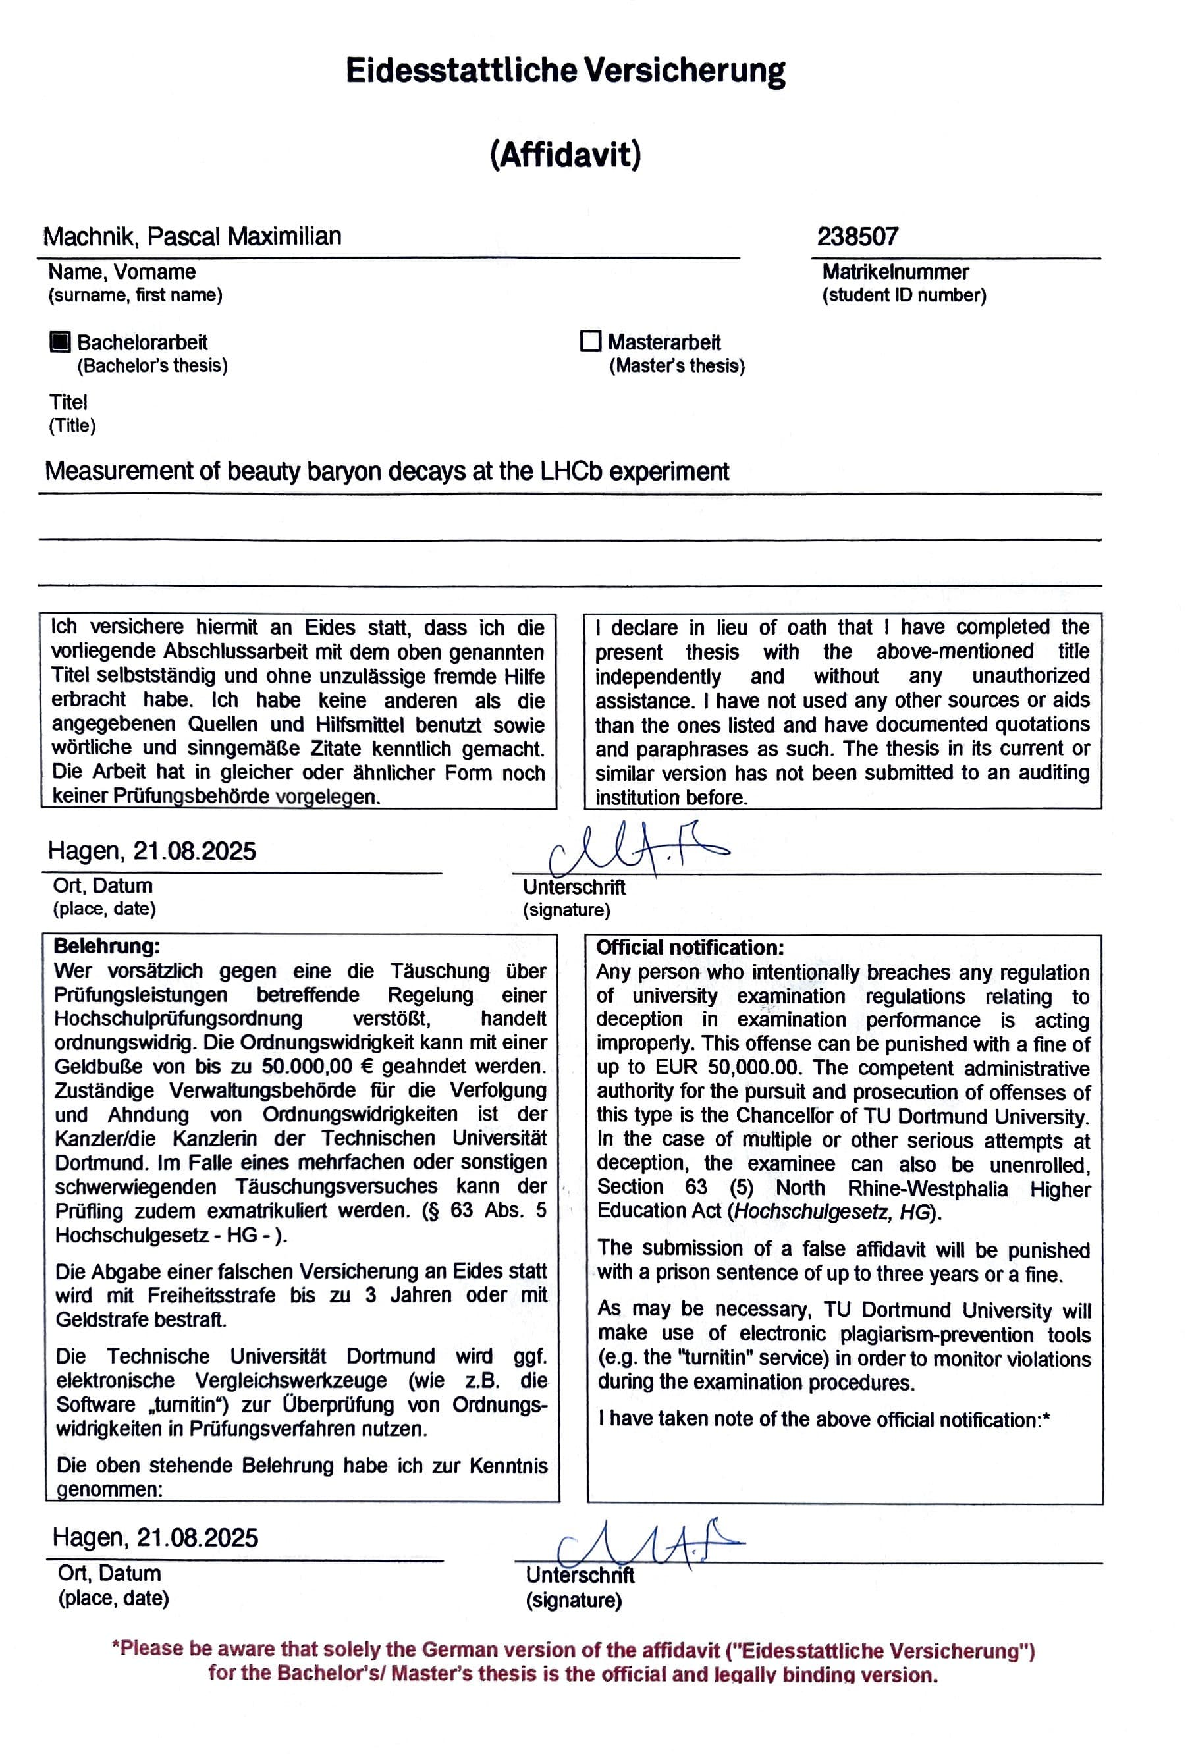
\includepdf{content/Eidesstattliche_Versicherung.pdf}

\end{document}
